\documentclass[12pt, a4paper]{report}
\usepackage[utf8]{inputenc}
\usepackage{titling} 
\usepackage{enumitem} 
\usepackage{graphicx} 
\usepackage{gensymb}
\graphicspath{ {./images/} } 

% if you want to create a new list from scratch
\newlist{alphalist}{enumerate}{1}
% in that case, at least label must be specified using \setlist
\setlist[alphalist,1]{label=\textbf{\alph*.}}

\setlength{\droptitle}{-10em}   % This is your set screw

\title{A REPORT \\ on \\[0.5in]\textbf{ALGORITHM DESIGN TO CONSTRUCT LARGE VESICULAR STRUCTURES IN AUTOPHAGY PATHWAY} \\~\\ Suchismita Tripathy \\ 2019A7PS0554P \\[1in] \textbf{Council of Scientific and Industrial Research - Institute of Genomics and Integrative Biology} \\
A Practice School – 1 Station of \\[0.75in] BIRLA INSTITUTE OF TECHNOLOGY AND SCIENCE PILANI } 
% \author{Suchismita Tripathy \\ 2019A7PS0554P}
\date{\vspace{-2.0cm}June 2021} 

\begin{document} 
\maketitle 

\section*{Acknowledgements}

I would like to take this opportunity to express my sincere gratitude to all the people who have supported me during the course of this project. I would like to thank BITS Pilani and CSIR-IGIB for giving me, as well as the other 18 students, the opportunity to work and learn at this institute for our PS-I. I would particularly like to thank Dr. Jyoti Yadav for her help with this, and for making us feel welcome from the very first day.\\~\\


Further, I would like to thank Dr. Lipi Thukral, my mentor for her guidance and for this opportunity to work under her with her team on autophagy. She has provided us with the necessary resources to help us gain insight into this project, and her explanations of her often intimidating work have been easy to understand for us students who do not have as much knowledge or experience in the field of biology. She has always been available for clearing our doubts and giving further pointers on the way forward, all while increasing our motivation for our work. Saman Fatihi and Pranav Ballaney, from the Phagophore team, have also been extremely helpful, providing explanations whenever I needed them and I am particularly thankful for their help. \\~\\


I would also like to thank our faculty mentor, Dr. Gautam Singhvi for his continuous motivation and support. He has been guiding us constantly in our PS-I journey so that we maintain discipline in our work and make the best out of this opportunity, by learning and doing as much as possible. We are all thankful to him for the same. 

\newpage

\begin{center} \textbf{BIRLA INSTITUTE OF TECHNOLOGY AND SCIENCE PILANI 
RAJASTHAN } 

Practice School Division 
\end{center}


\textbf{Station:} Council of Scientific and Industrial Research – Institute of Genomics and Integrative Biology 
\\\textbf{Duration:} 2 months                         \\\textbf{Date of Start:} 31st May 2021 
\\\textbf{Date of Submission:} 23rd June 2021 
\\~\\\textbf{Project Title:} Algorithm Design to construct large vesicular structures in autophagy pathway 
\\~\\
\textbf{Name:} Suchismita Tripathy 
\\\textbf{ID:} 2019A7PS0554P 
\\\textbf{Discipline:} Computer Science 
\\~\\
\textbf{Mentor Name:} Dr. Lipi Thukral 
\\\textbf{Designation:} Sr. Scientist | Computational Structural Biology
\\\textbf{E-mail:} lipi.thukral@igib.in 
\\~\\
\textbf{Name of PS Faculty:} Dr. Gautam Singhvi 
\\\textbf{E-mail:} gautam.singhvi@pilani.bits-pilani.ac.in 
\\~\\
\textbf{Key Words: }GROMACS, Curved lipid bilayers, Autophagy pathway, Phagophores, Double membrane vesicles 
\\\textbf{Project Areas:} Molecular Dynamics Simulations, Autophagy
\\~\\~\\
\textbf{Abstract:} There is growing focus on autophagy as a research area with its links to preventing and curing cancer. The formation of the autophagosome as a double membrane vesicle is vital to the degradation of unwanted cellular components and this process involves curved membrane configurations, as the phagophore is formed de novo. The simulation of this would hence require careful calculations to ensure stability in complex topologies and would further require protein embedding on the surface of the vesicle. 

\clearpage 
% \hspace{-3.5cm}
% \includegraphics[width=20cm]{images/nda image.png} 

\newpage 
\tableofcontents

\newpage 
\section*{Introduction}
\addcontentsline{toc}{section}{Introduction}

The autophagy pathway involves the formation of a phagophore (controlled by the Atg genes) which expands through the addition of lipids to its membranes to form an autophagosome which later fuses with a lysosome to degrade a part of the cytoplasm. This formation process involves different shapes and structures as the phagophore progresses to form a closed vesicle like the C and Half-O shapes. In addition, this vesicle has a double-membrane. The simulation of single bilipid layers has been achieved by the BUMPy (Building Unique Membranes in Python) tool which allows the formation of curved configurations and topological states more complex than flat bilayers, by dealing with the consequences of increasing complexity on the physical properties of the system (like interleaflet ratio, the differing number of lipids in the curved leaflets). This project aims first at gaining comprehensive knowledge of the formation of phagophores and their stages of growth, the nature of the lipid bilayers and double membranes, algorithms like BUMPy that simulate membranes and vesicles and the proteins that are part of such structures. Using this information, I will try to design functions for the careful embedding of proteins on the double layer membranes of phagophores for molecular dynamics simulations. \\~\\


\subsection*{Project Details} 
\addcontentsline{toc}{subsection}{Project Details}

\textbf{Title:} Algorithm Design to construct large vesicular structures in autophagy pathway 
\\~\\
\textbf{Mentor: }Dr. Lipi Thukral 
\\\textbf{Faculty Mentor:} Dr. Gautam Singhvi 
\\~\\
\textbf{Skill Set Required:} Experience in Python, Experience with NumPy and SciPy (dependencies of BUMPy), Experience with MDAnalysis
\\~\\
% \textbf{Expected Outcomes: }Algorithm for the formation of different stages in the development of a phagophore with proeprly embedded proteins 
% \\~\\~\\
% \textbf{Initial Work Plan and Milestones:}
% \\ 
% \begin{enumerate}
% \item Learning and exposure to relevant concepts through available research papers and existing tools – Week 2 (14th June 2021) 
% \begin{alphalist}
% \item Structure of lipid bilayers, individual molecules and the effects that curvature can have on the placement/number/orientation of the molecules and the dimensions of the membrane  
% \item Autophagy Pathway and vesicle structures involved, particularly the structures a phagophore goes though in its biogenesis as it starts from a nucleate to a closed, spherical autophagosome  
% \item BUMPy algorithm and the way it simulates the bilayer, deals with the effects of complex geometries on the physical properties 
% \item Other tools for MD simulations that simulate lipid bilayers and vesicles that may help provide insight, like CHARMM-GUI coarse-grained vesicle builder, LipidWrapper 
% \end{alphalist}
% \item Algorithm Design and Evaluation – Week 4 (28th June 2021) 
% \item Implementation in Python – Week 6 (12th July 2021) 
% \item Testing and Optimisation – Week 7 (19th July 2021) 
% \item Report Writing – 23rd July 2021 
% \end{enumerate}
	

% Modifications will be made to this and the work plan will be changed based on new requirements and inputs from my mentor as well. 

% \newpage 
% \section*{Organisation Information} 
% \addcontentsline{toc}{section}{Organisation Information} 

% \textbf{Basic Hierarchy:} 
% \\
% -$>$ Ministry of Science and Technology 
% \\ 
% -$>$ Department of Scientific and Industrial Research 
% \\ 
% -$>$ Council of Scientific and Industrial Research 
% \\ 
% -$>$ Institute of Genomics and Integrative Biology 

% \subsection*{Council of Scientific and Industrial Research} 
% \addcontentsline{toc}{subsection}{Council of Scientific and Industrial Research}

% CSIR was set up by the Government of India in 1942 and has become the leading centre for research in India, with 37 laboratories under its helm across different states, including 39 outreach centres, 3 Innovation Complexes, and five units with a pan-India presence. It has also made great strides in Intellectual Property, with a patent portfolio of 1,132 unique patents in force, out of which 140 patents have been commercialized, along with publishing many papers (5009 in SCI journals in 2019). 
% \\~\\
% -	\textbf{Vision:} “Pursue science which strives for global impact, technology that enables innovation – driven industry and nurture trans-disciplinary leadership thereby catalyzing inclusive economic development for the people of India.” 
% \\~\\
% -	\textbf{National Labs:} 
% \begin{enumerate}
%     \item AMPRI - Advanced Materials and Processes Research Institute 
%     \item CBRI - CSIR-Central Building Research Institute 
%     \item CCMB- Centre for Cellular and Molecular Biology 
%     \item CDRI - Central Drug Research Institute 
%     \item CECRI- Central Electro Chemical Research Institute 
%     \item CEERI - Central Electronics Engineering Research Institute 
%     \item CFTRI - Central Food Technological Research Institute 
%     \item CGCRI - Central Glass and Ceramic Research Institute 
%     \item CIMAP - Central Institute of Medicinal and Aromatic Plants 
%     \item CIMFR - Central Institute of Mining and Fuel Research 
%     \item CLRI - Central Leather Research Institute 
%     \item CMERI - Central mechanical engineering research institute 
%     \item CRRI - Central Road Research Institute 
%     \item CSIO - Central Scientific Instruments Organisation 
%     \item CSMCRI - Central Salt and Marine Chemicals Research Institute 
%     \item IGIB - Institute of Genomics and Integrative Biology \item IHBT - Institute of Himalayan Bioresource Technology 
%     \item IICB - Indian Institute of Chemical Biology 
%     \item IICT - Indian Institute of Chemical Technology 
%     \item IIIM, Jammu - Indian Institute of Integrative Medicine 
%     \item IIP - Indian Institute of Petroleum 
%     \item IMMT - Institute of Minerals and Materials Technology 
%     \item IMTECH - Institute of Microbial Technology 
%     \item IITR - Indian Institute of Toxicology Research 
%     \item NAL - National Aerospace Laboratories 
%     \item NBRI - National Botanical Research Institute 
%     \item NCL - National Chemical Laboratory 
%     \item NEERI - National Environmental Engineering Research Institute 
%     \item NEIST (RRL), Jorhat - North East Institute of Science and Technology, Jorhat 
%     \item NGRI - National Geophysical Research Institute 
%     \item NIIST - National Institute for Interdisciplinary Science and Technology 
%     \item NIO - National Institute of Oceanography 
%     \item NISCAIR – National Institute of Science Communication and Information Resources 
%     \item NISTADS – National Institute of Science Technology and Development Studies 
%     \item NML - National Metallurgical Laboratory 
%     \item NPL - National Physical Laboratory 
%     \item SERC - Structural Engineering Research Centre 
% \end{enumerate}

% % \\~\\
% -	\textbf{Organisation Structure:} 

% \begin{figure}[h]
%     \centering 
%     \includegraphics[scale=1]{images/org structure.png} 
%     \centering 
%     \caption{Organisation Structure at CSIR} 
% \end{figure} 

% -	\textbf{Director General:} Shekhar C. Mande. 
% \\ 
% Each laboratory under CSIR has their own Director as well. 

% \subsection*{Institute of Genomics and Integrative Biology} 
% \addcontentsline{toc}{subsection}{Institute of Genomics and Integrative Biology}

% Initially established as the Centre for Biochemical Technologies in 1977, this research institute was renamed to IGIB in 2002 after a Functional Genomics Unit was established in 1988, with an increasing focus on genomics over biochemistry. IGIB carried out the first re-sequencing of the human genome in India, while also being involved in the sequencing of Sri Lankan and Malaysian genomes. 
% With the COVID-19 pandemic, IGIB has played a pivotal role by helping increase the accuracy of the sequencing of the SARS-CoV-2 genome, which further facilitated the quick implementation of policies regarding the pandemic by the government. Its scientists also identified a new clade of SARS-CoV-2 in India and developed a new testing method called FELUDA based on CRISPR gene editing, that has been licensed for commercial production as well. 
% \\~\\ 
% -	\textbf{Mission:} "To translate concepts developed in basic biological research to commercially viable technologies for health care." 
% \\~\\
% -	\textbf{Research Focus:} CSIR – IGIB focuses on the following areas of research: 
% \begin{enumerate}
%     \item Genomics and Molecular Medicine: Collaborative projects like the Indian Genome Variation Consortium and exploring the genetics of neuropsychiatric disorders like schizophrenia and diabetes and other complex disorders 
%     \item Cardio-Respiratory Disease Biology: Research on Chronic Obstructive Pulmonary Disorder, tuberculosis and asthma and related allergies 
%     \item Chemical and Systems Biology: Biochemical research on areas including nanobiotechnology, novel assay methods, and new molecules 
%     \item Informatics and Big Data: High-throughput data analysis and gene annotation, genome informatics 
%     \item Integrative and Functional Biology: Involves understand the mechanisms, particularly at the molecular level, of complex disorders like neurological diseases, cancer, diabetes and skin diseases 
% \end{enumerate} 

% % \\~\\
% -	\textbf{Director:} Anurag Agrawal 
% \\ 
% The faculty includes Chief Scientists, Senior Principal Scientists, Principal Scientists, Senior Scientists and Scientists. 


\newpage 
\section*{Background Information} 
\addcontentsline{toc}{section}{Background Information}


Since this is quite a niche topic, a significant amount of research was required to at least get to the point where the way forward and the deliverables can be assessed realistically, and then worked upon, using the various tools that may be required. For this, I chose to focus on the following topics to understand the keywords of this project, through research papers and other sources on the Internet: 
\\~\\ 
\begin{enumerate}
\item Structure of lipid bilayers, individual molecules and the effects that curvature can have on the placement/number/orientation of the molecules and the dimensions of the membrane 
\item Autophagy Pathway and vesicle structures involved, particularly the structures a phagophore goes though in its biogenesis as it starts from a nucleate to a closed, spherical autophagosome 
\end{enumerate}

In the following few pages, I will elaborate on the knowledge I have gained through the literature review pertaining to autophagy. \\~\\


\subsection*{Lipids} 
\addcontentsline{toc}{subsection}{Lipids}

Lipids are the building blocks of membranes, the focus of this project. They are macro biomolecules and their common examples include oils, waxes, fatty acids, fat soluble vitamins (A, D, E and K), monoglycerides, diglycerides, triglycerides, phospholipids and even hormones. Lipids consist of hydrocarbons in their most reduced form which is why they are also an excellent form of energy storage (when metabolized the hydrocarbons oxidize to release large amounts of energy), in addition to helping with the structure of cells as part of membranes. As lipids are non-polar, they are not soluble in water but are soluble in non-polar solvents like chloroform. 
\\~\\
The amphiphilicity of phospholipids (a class of lipids) is what leads them to form the vesicles and membranes that are so prominent in cells, along with other proteins, with their hydrophilic heads and 2 hydrophobic fatty-acid chains. Depending on the location and use of the membrane itself, lipids can form 20\% - 80\% of the membrane, with the rest being proteins. There are a variety of lipids that can be used to make bilayers, including: 
\begin{enumerate}
\item POPC: 1-palmitoyl-2-oleoyl-sn-glycero-3-phosphocholine
\item DOPC: dioleoyl-phosphatidylcholine
\item POPI: 1-palmitoyl-2-oleoyl-sn-glycero-3-phosphoinositol
\item DPPC: dipalmitoyl-phosphatidylcholine
\end{enumerate}


\begin{figure}[h]
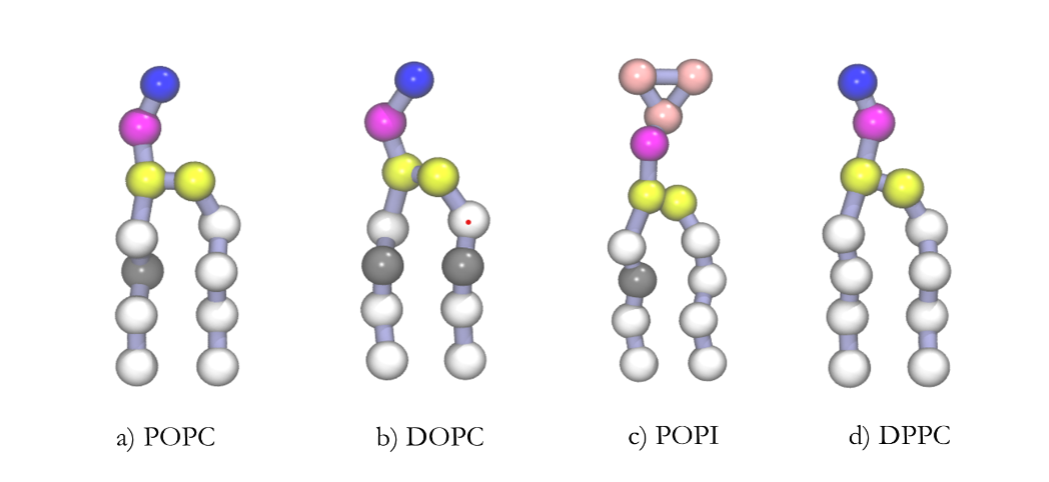
\includegraphics[scale=0.5]{images/lipids with labels.png} 
\centering 
\caption{Phospholipids} 
\centering 
\end{figure} 


\subsection*{Lipid Bilayers} 
\addcontentsline{toc}{subsection}{Lipid Bilayers} 

Lipid bilayers are continuous membranes that surround the cells of almost all organisms and many viruses, including the cell nucleus and other membrane-bound organelles. This semi-permeable membrane is the barrier that keeps ions, proteins and other molecules in place by preventing them from crossing the membrane through diffusion (transport of some elements across the membrane is carried out with the help of membrane proteins instead, often called ion pumps). They are impermeable to hydrophilic (water-soluble) molecules and particularly to ions and are only a few nanometers wide.
\\~\\
As mentioned before, the lipids that make up these bilayers are phospholipids which are amphiphilic i.e. both hydrophilic (water-loving) and lipophilic (fat-loving). They thus arrange themselves into bilayers by forming a sheet-like structure with two levels, or leaflets. In each layer, the lipophilic chains of each molecule are oriented toward the same side, and when both layers are put together, the lipophilic chains can all be seen in the middle. Their polar or hydrophilic heads are thus positioned towards the outside i.e. towards the aqueous medium. Thus, the inside of the bilayer sheet is a non-polar region sandwiched between the two polar sheets.  Phospholipids with certain head groups can also alter the surface chemistry of a bilayer and can, for example, serve as signals as well as "anchors" for other molecules, yet another use of lipids in the biological system. The packing of lipids within the bilayer also affects its mechanical properties, including its resistance to stretching and bending, importance for curvature and complex shapes that may need to be simulated for various purposes. 
\\~\\
\begin{figure}[h]
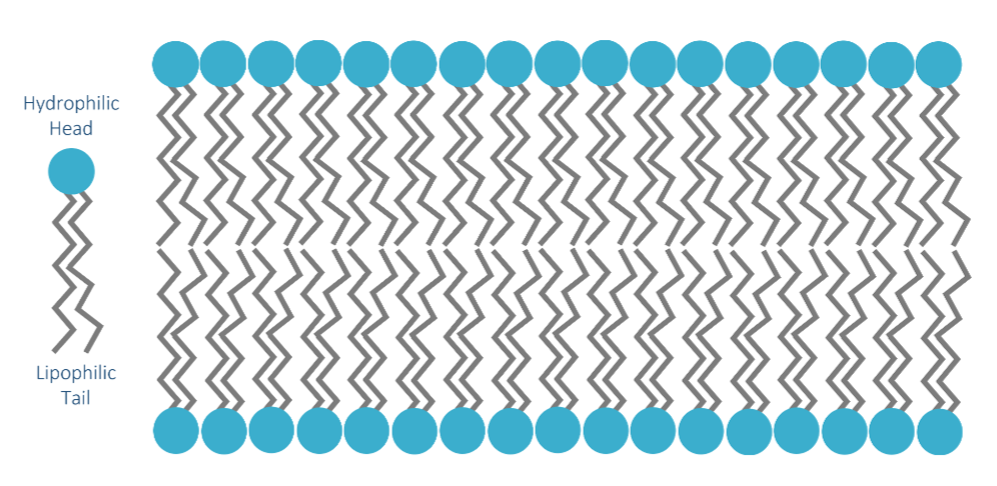
\includegraphics[scale=0.5]{images/lipid bilayer custom.png} 
\centering 
\caption{Lipid Bilayer} 
\centering 
\end{figure} 
\\~\\ 
Bilayers, being fragile and invisible in traditional microscopy, are usually studied using electron or atomic force microscopy. \\~\\


\subsection*{Autophagy} 
\addcontentsline{toc}{subsection}{Autophagy} 


The name autophagy comes from the Ancient Greek word autóphagos which means ‘self-devouring’ and refers to the natural, controlled cellular mechanism for the degradation of unnecessary or dysfunctional components and even cells as a whole, the ‘waste-disposal system’ of the cell. The process involves isolating the cellular matter that must be broken down, transporting it to the lysosome, degradation by hydrolytic enzymes and re-utilisation of the degradation products. As explained to us by our mentor, autophagy plays a vital role in times of starvation, by breaking down cellular material and reusing it for cellular processes, while nourishment is found (in the case of yeast, nitrogen starvation is the greatest factor that results in autophagy). Apart from starvation adaptation, autophagy is also important for maintaining the homeostasis of non-starved cells, which involves: 
\\
\begin{enumerate}
\item Recycling residual proteins 
\item Enabling regeneration of cellular components 
\item Anti-ageing 
\item Removal of microorganisms (xenophagy) 
\item Antigen Presentation 
\item Programmed Cell Death (PCD)  
\item Removal of toxic proteins from cells that are involved in neurodegenerative diseases like Parkinson’s and Alzheimer’s 
\item Recognition and removal of cancer cells and others that could harm the body (tumor suppression)
\end{enumerate} 

There has recently been a lot of focus on the role of autophagy in preventing/treating cancer (autophagy can also promote the survival of tumor cells by not acting on them), that has resulted in many studies on the autophagy pathway and the genes that control this mechanism, in the hopes of finding new information that could help in the fight against cancer. 
\\~\\~\\
There are 4 kinds of autophagy: 
\begin{enumerate}
    \item Macroautophagy 
    \item Microautophagy 
    \item Chaperone-Mediated Autophagy 
    \item Crinophagy 
\end{enumerate} 


Macroautophagy is the most researched form of autophagy and also the form that this project is concerned with. Here, the cytoplasmic content that needs to be removed is isolated in an autophagosome, a double-membrane vesicle, which later fuses with a lysosome for the final break down of its contents. This process of autophagosome formation is what this project aims to simulate, by being able to build the required files for the concerned vesicle shapes for GROMACS to then work on. 
\\~\\~\\~\\
\textbf{Autophagosome Formation:} Broadly, this process starts with the formation of a phagophore, the initial sequestering organelle, that grows and expands with the acquisition of lipids and then forms a closed, double-membrane vesicle around the targeted cell component, forming the autophagosome. This autophagosome (average diameter of 700nm), when fused with a lysosome (vesicles carrying the special hydrolytic enzymes required for the degradation process) forms what is then called the autolysosome. The autophagosome is thus formed de novo, not through fission or fusion. 
\\~\\
There is not a lot that is known of this formation pathway with certainty, but many theories based on some empirical evidence have been put forward, with conflicting ideologies that still exist today because unlike yeast (where phagophore formation starts at a phagophore assembly site), in mammalian cells this formation is more unpredictable. Autophagosome biogenesis is known to start with omegasomes, a sub-domain of the endoplasmic reticulum (ER membrane), following autophagy induction. They are cell compartments with lipid bilayer membranes enriched with the phospholipid phosphatidylinositol 3-phosphate (PtdIns3P) and are named for their resemblance to the Greek letter $\omega$ (omega). Specific receptor proteins recruit items for phagophore formation from here, while the phagophore slowly expands. The ER membrane (specifically, the mitochondria associated ER membrane or MAM) thus forms the platform for phagophore formation, where certain puncta and markers collect to initiate the process. Lipids move from the ER membrane to the growing phagophore, including, possibly, mitochondrial proteins that have been found on autophagosome surfaces. During this phase of rapid growth, the phagophore is known to attain a maximum diameter of 1000nm. 
\\~\\
However, including the ER membrane, other sites have been though of as being the starting sites of phagophore formation, including the Golgi apparatus and the plasma membrane itself, from where lipids could also be procured. It is further possible that the procurement of lipids takes place from multiple sources and not a single one. Autophagosomes further have a very low concentration of proteins, as compared with other membranes and are richer in lipids instead. 
\\~\\
As seen in the below diagram, the autophagosome formation process involves a number of different shapes and curvatures of the lipid bilayer double-membranes, including a C and a half-O shape, apart from the final full sphere. After this, as the lysosome fuses with autophagosome to form the autolysosome, the shape of the structure changes again, and the point of fusion, where a tube-like structure is formed, is cylindrical, joining the 2 partial spheres of differing diameter on either side. Thus, simulating this process will require the simulation of all the shapes, including possible toroidal shapes as required for the ER membrane wherein phagophore formation begins.
\\~\\
\begin{figure}[h]
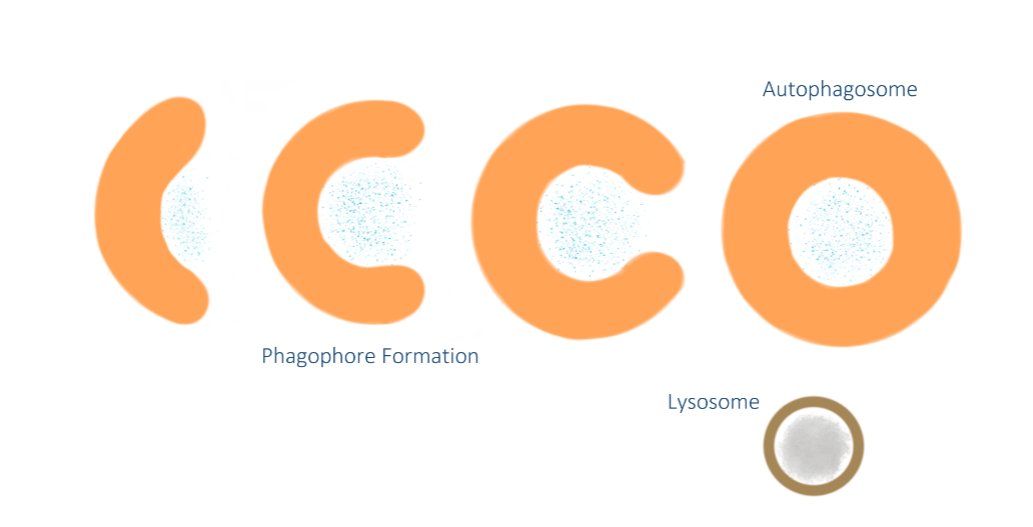
\includegraphics[scale=0.5]{images/autophagy stages.png} 
\centering 
\caption{Stages and Structures in Phagophore Formation} 
\centering 
\end{figure} 

The formation of autophagosomes is controlled by a collection of genes, including the Atg genes (Atg12-Atg5) and LC3 complexes. Considerable research was carried out on the genes involved in autophagy and presented in the paper ‘Human LC3 and GABARAP subfamily members achieve functional specificity via specific structural modulations’ by Nidhi Jatana, David B. Ascher, Douglas E.V. Pires, Rajesh S. Gokhale and Lipi Thukral. Though some of the in-depth information in this paper would not be required for this project, some of the interesting details from this paper are discussed here. 
\\~\\~\\~\\
\textbf{Proteins involved in autophagy:} In yeast, the formation of the double-membrane autophagosomes is controlled by the single Atg8 protein. This protein has developed into a group of 6 related proteins in humans (orthologs): LC3A, LC3B, LC3C, GABARAP, GABARAPL1, and GABARAPL2/ GATE16, thus grouped into the LC3 and GABARAP families. It is known that the LC3 family (of which the LC3B protein is a part and is also the most studied of the human Atg8 protein group) controls the elongation of the phagophore membrane, while the GABARP family is mostly involved in sealing the autophagosome at the end. 
\\~\\
The aforementioned paper studied the evolutionary and sequence relationships between the Atg8 homologs, showing how most of the proteins share very few similarities, with the highest similarities existing between LC3A-LC3B and GABARAP-GABARAPL1. The distinct binding sites, binding patterns, changes in terminal groups, non-covalent bonding like hydrogen bonding along with protein dynamics in PLEKHM-1 bound state (peptide) were further studied to properly distinguish the different members of the protein families and ascribe functions to each. 
\\~\\
The mutations related to these proteins that caused cancer were also researched, highlighting the importance of autophagy research in the global fight against cancer. Out of the 373 mutations in the 6 proteins, 174 were classified as being disease-related, with more than 50\% being classifies as having considerable impact on health. 43 mutations were found to be related to cancer, with endometrial cancer being the most prevalent form related to mutations in all the proteins. Mutations in the human Atg8 orthologs were linked to various cancers as follows: 
\begin{enumerate} 
\item LC3A – Bladder Cancer 
\item LC3B – Lung Cancer 
\item LC3C – Prostate and Skin Cancers 
\item GABARAP – Thymic Cancer 
\item GABARAPL1 – Stomach Cancer 
\item GABARAPL2/GATE1 – Breast Cancer 
\end{enumerate} 

\clearpage
A picture of the crystal structures of the proteins is shown here, adapted from an image made available in the same paper: 
\begin{figure}[h]
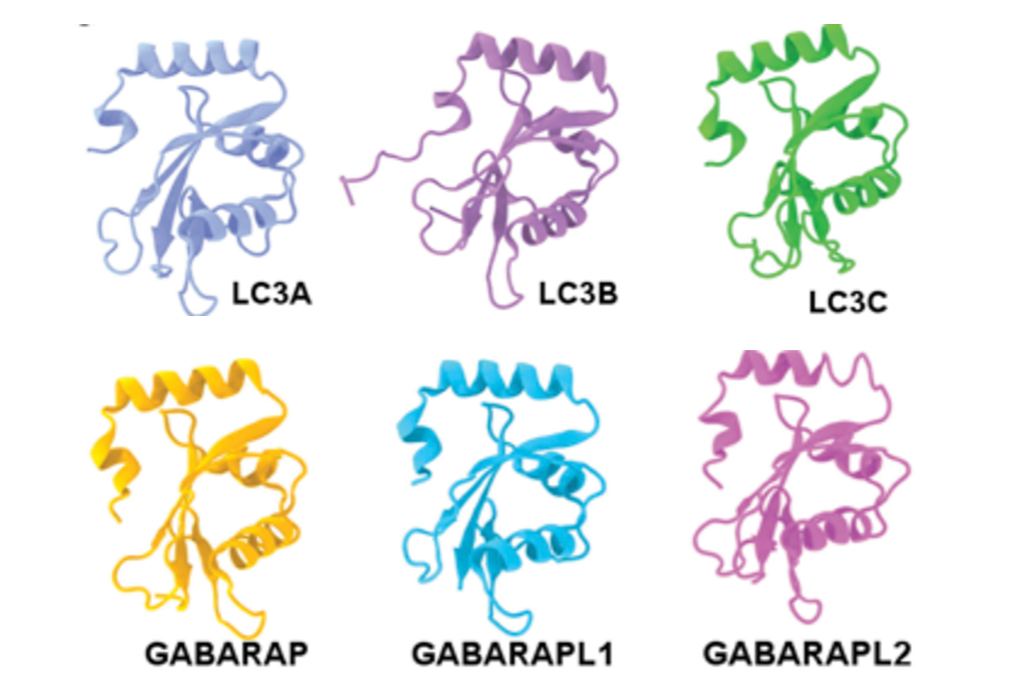
\includegraphics[scale=0.5]{images/atg.png} 
\centering 
\caption{Atg8 Orthologs} 
\centering 
\end{figure} 

\clearpage 
\section*{Tools} 
\addcontentsline{toc}{section}{Tools} 

In addition to the background theory research, since this project involves and expands on existing tools in the realm of molecular dynamics simulations, I had to familiarize myself with a variety of tools, and get some hands-on experience. I looked into Chimera, MARTINI and the tool BUMPy (Building Unique Membranes in Python) which allows the formation of curved configurations and topological states more complex than flat bilayers, by dealing with the consequences of increasing complexity on the physical properties of the system. I also had to familiarize myself with GROMACS, the basic tool used for molecular dynamics simulations, to understand how BUMPy, a command line tool, fits in with this and is able to produce outputs in the required file formats for GROMACS to work on and thus simulate the required shapes and systems. Finally, I looked into and familiarised myself with MDAnalysis as well. 
\\~\\~\\
\textbf{Molecular Dynamics:} Molecular dynamics is a computer simulation method for visualizing and analysing the physical movement of atoms and molecules, in different environments and conditions, to study their behaviour. The atoms are allowed to interact for a given period of time (usually specified in nanoseconds, the value can vary from simulation to simulation) and the trajectories of the particles are calculated by solving numerically Newton’s equations of motion, taking into account all the inter-atomic forces and potential energies. The systems studied are of varying sizes: quantum (lowest), all-atom, coarse-grained, mesoscale (highest). 
\\~\\~\\~\\ 
\subsection*{Chimera} 
\addcontentsline{toc}{subsection}{Chimera} 


For the visualization of biomolecules, there are a variety of tools available including pymol and VMD (Visual Molecular Dynamics). UCSF Chimera is such a program for the interactive visualization of biomolecules and trajectories developed by the Resource for Biocomputing, Visualization, and Informatics (RBVI) at the University of California, San Francisco. It can be used as both a command line tool or through menus and commands. The molecules can be visualized through .pdb files, which are the inputs to this software. PDB stands for Protein Data Bank and is a textual file that contains information of the coordinates and 3-dimensional structures of molecules. These files can be found on the Research Collaboratory for Structural Bioinformatics PDB site, as well as other sources. After the completion of an MD simulation, the final trajectory can be converted to .pdb file format as well for final visualization. An example of a visualization of a protein using Chimera is shown here, that I used while carrying out a tutorial: 
\\~\\ 
\begin{figure}[h]
    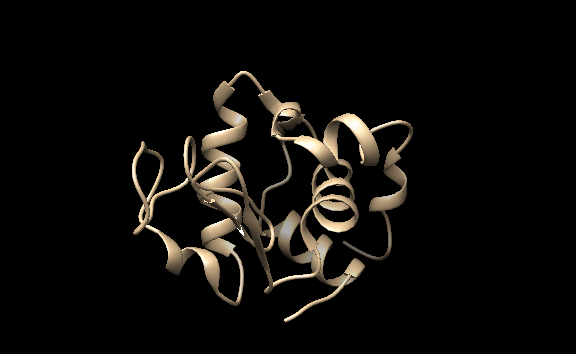
\includegraphics[scale=0.9]{images/hen egg white lysosyme.png} 
    \centering 
    \begin{center} \caption{The Structure of the Orthorhombic Form of Hen Egg-White Lysozyme at 1.5 angstroms Resolution, as viewed in Chimera} 
    \centering 
    \end{center} 
\end{figure} 


\subsection*{GROMACS} 
\addcontentsline{toc}{subsection}{GROMACS} 


GROMACS is one of the most widely-used packages for molecular dynamics simulations, mainly built to simulate proteins, lipids and nucleic acids. It was developed at the Biophysical Chemistry department at the University of Groningen and can run on local CPUs as well as GPUs. Some of the main file formats used as inputs in GROMACS are (other than .pdb): 
\\~\\ 
\begin{enumerate}
    \item .top: This file contains all the information necessary to define a molecule within a simulation, and hence specifies molecular topology. It is often the main entry-point in the GROMACS pipeline. 
    \item .itp: ‘itp’ here stands for ‘include topology’. These files are generally made and used for molecules that are very common in the simulations being carried out. They are included into the .top files using a ‘\#include’ statement at the top, and their usage drastically shortens the length of the .top files. Each .itp file can contain more than one molecule definition: some of the .itp files available on MARTINI have collections of lipids, or solvents like water and antifreeze. 
    \item .gro: These are also known as coordinate files and they contain information on the molecule structure. They are not always necessary and can be switched with certain other file formats also. 
    \item .mdp: These files contain molecular dynamics simulation parameters and are generally used to run energy minimization (a process to relax the system by ensuring that the system has no steric clashes or inappropriate coordinates) or the MD simulations. 
    \item .tpr: It is a portable binary run input file, which contains the starting structure of the simulation along with the topology and other parameters (combining the data in the above files). 
\end{enumerate} 


GROMACS is operated via a command-line interface and has a number of tools that are commonly used (as modules of ‘gmx’), including: 
\\~\\ 
\begin{enumerate} 
\item pdb2gmx: This module reads a .pdb (or .gro) file along with some database files and then adds hydrogens to the molecules for generating coordinates. It thus takes a .pdb file as input to produce a .top file, usually named topol.top, and also produces a position restraint and post-processed structure file. 
\item solvate: A simulation is run by defining a simulation box and filling it with solvent. This solvation is accomplished by solvate, with the required coordinate files (.gro) and also the .top file. 
\item grompp: This is the preprocessor in GROMACS that reads a molecular topology file and expands its topology from a molecular description to an atomic description after checking its validity. 
\item mdrun: This is the main computational chemistry engine within GROMACS. It performs the following functions: molecular dynamics simulations, stochastic dynamics, energy minimization, test particle insertion calculation/recalculation of energies. 
\end{enumerate} 

Using these command-line tools, molecular dynamics simulations can be carried out by creating .top files, creating a simulation box, carrying out the necessary energy minimisations/equilibriations and solvation and final assembly. 
\\~\\
For getting familiar with GROMACS, I tried out the hen egg-white lysozyme tutorial by Justin Lemkul but could only run it till the second last command. This was because I was working on a VM and the processing power of my own laptop could not handle the command itself. \\~\\ 


\subsection*{BUMPy} 
\addcontentsline{toc}{subsection}{BUMPy} 


BUMPy (Building Unique Membranes in Python) is a tool for generating curved bilayer configurations. Most of the available bilayer building tools only generate flat bilayers, while BUMPy deals with the practical complications related with increasing complexity and curvature to ensure that the resulting structure has no inappropriate coordinates or uneven numbers of lipids. It functions by taking a pdb file as input (for a flat bilayer) and then performs its calculations on the related parameters to produce a .top file, which can then be used further as the input to GROMACS, with other files as well. One of the most important issues in curved bilayers is that of interleaflet ratios – a bilayer normally has the same number of lipids in the upper and lower layers (or leaflets) while on being curved, due to surface-area mismatch, there is a change in the number of lipids in each leaflet (the outer one will have more). This tool uses the concept of a monolayer pivotal plane (a surface within the monolayer that has the same surface area in both flat and curved systems) for calculating the interleaflet ratios and numbers of lipids. There are further calculations that vary for each shape supported, which are: 
\\~\\ 
\begin{enumerate}
    \item Cylinders 
    \item Spheres 
    \item Semi-spheres 
    \item Tori 
    \item Partial tori 
    \item Double bilayer cylinder 
    \item Semi-cylinder plane 
    \item Semi-sphere plane 
    \item Capped cylinders 
\end{enumerate} 

\begin{figure}[h]
    \includegraphics[scale=0.75]{images/bumpy.png} 
    \centering 
    \caption{Coordinates and structure of a flat bilayer and the a semi-cylinder as adapted from “BUMPy: A Model-Independent Tool for Constructing Lipid Bilayers of Varying Curvature and Composition.”} 
    \centering
\end{figure} 


\newpage
\subsection*{MARTINI} 
\addcontentsline{toc}{subsection}{MARTINI}  


MARTINI is a coarse-grained force field for molecular dynamics simulations with a four-to-one mapping (4 heavy atoms and their associated hydrogens are represented by only one interaction centre). It was also developed at the University of Groningen and was initially made only for the simulation of lipids. Parameters for a large number of molecules are available including basic particle definitions (like water), amino acids, sugars, ions, solvents, DNA, RNA, polymers and of course lipids. There are also topology and coordinate files available apart from the .itp files. 

Building a bilayer: Using the MARTINI files available, I tried building a simple lipid bilayer myself on my VM. I thus learnt about the pipeline and the necessary file formats for each step: 
\\~\\ 
\begin{enumerate}
    \item .itp files for the required lipid and water (particle definitions): Create a .top file for the layer itself by including these two files: 
    \\~\\
    \#include "martini\_v2.1.itp" //for water (W)
    \\
    \#include "martini\_v2.0\_DPPC\_01.itp" // for the lipid
    \\~\\
    {[ system ]}
    \\DPPC BILAYER SELF-ASSEMBLY
    \\~\\
    {[ molecules ]}
    \\DPPC 128
    \\; W 768 
    \\~\\ 
    
    \item Coordinates for a single lipid molecule and for water as well (DPPC-em.gro and water.gro) 
    \item Creating a simulation box containing a random configuration of the lipids using the insert-molecules command, in the case of DPPC being: 
    \\~\\ 
    gmx insert-molecules -ci DPPC-em.gro -box 7.5 7.5 7.5 -nmol 128 -radius 0.21 -try 500 -o 128\_noW.gro 
    \item 
    A minimization.mdp settings file for a short energy minimization of the system for getting rid of high forces between beads that may have been placed quite close to each other. This is done using the grompp tool (the gromacs preprocessor that reads a molecular topology file, checks its validity and expands the topology from a molecular description to an atomic description) and the mdrun tool. 
    \item Using the solvate tool, water molecules are added, the .top file is updated to reflect the number of water molecules (calculated from the waterbox.gro file) and a second round of energy minimization is carried out. 
    \item Finally, the self-assembly MD simulation can be run, using also the martini\_md.mdp file. As mentioned before, the final trajectory is converted to .pdb format for visualization. 
\end{enumerate} 


\textbf{Commands Used:} 
\\~\\
gmx insert-molecules -ci DPPC-em.gro -box 7.5 7.5 7.5 -nmol 128 -radius 0.21 -try 500 -o 128\_noW.gro 
\\(Creating a simulation box)
\\~\\
gmx grompp -f minimization.mdp -c 128\_noW.gro -p dppc.top -o dppc-min-init.tpr 
\\(First energy minimization)
\\~\\
gmx mdrun -deffnm dppc-min-init -v -c 128\_minimized.gro 
\\~\\
gmx solvate -cp 128\_minimized.gro -cs water.gro -o waterbox.gro -maxsol 768 -radius 0.21 
\\(Solvation)
\\~\\
gmx grompp -f minimization.mdp -c waterbox.gro -p dppc.top -o dppc-min-solvent.tpr  
\\(Second energy minimization)
\\~\\
gmx mdrun -deffnm dppc-min-solvent -v -c minimized.gro \\~\\
gmx grompp -f martini\_md.mdp -c minimized.gro -p dppc.top -o dppc-md.tpr 
\\~\\
gmx mdrun -deffnm dppc-md -v 
\\(Final self-assembly)
\\~\\ 
gmx trjconv -s dppc-md.tpr -f dppc-md.xtc -o dppc-md.pdb -pbc whole -conect 
\\(Conversion to pdb format)
\\~\\
Similar steps can be applied to other lipids, whose .itp files and .gro files (for coordinates) are readily available on the MARTINI website by writing the initial .top file and modifying others. 
\\~\\~\\

\begin{figure}[h]
    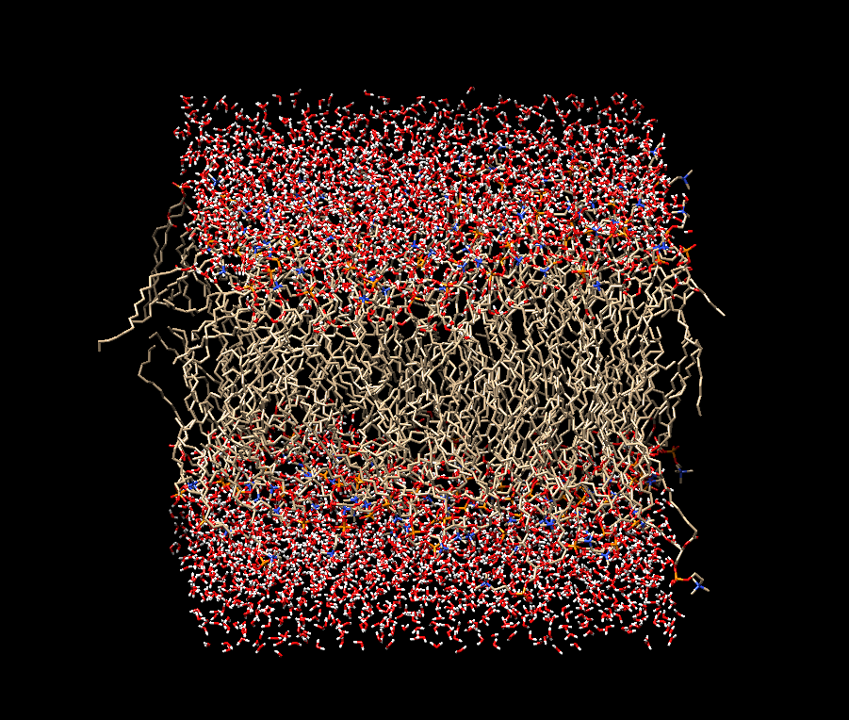
\includegraphics[scale=0.65]{images/dppc 128.png} 
    \centering 
    \caption{DPPC bilayer with 128 lipids, as obtained from the CHARMM-GUI website and viewed in Chimera}
    \centering
\end{figure} 


% Modifications to this process and the text files involved, as well as corrections will be carried out. 

% \newpage
\clearpage

\subsection*{MDAnalysis} 
\addcontentsline{toc}{subsection}{MDAnalysis} 

MDAnalysis is a Python library to aid in the analysis of MD simluation files and trajectories. It has a variety of methods to read MD simulation file formats (particle-based trajectories and individual coordinate frames like pdb files) and analyse the different residues, chains, atoms etc. in the files, viewing and changing coordinates of atoms (using NumPy arrays), calculating important reference points like centroids etc. and writing these to output files of the same formats. 
\\~\\ 
Since MDAnalysis is object-oriented, it heavily uses classes to deal with its functionality. Its primary class is 'MDAnalysis.core.Universe'. Reading files and extracting its data always starts with creating a universe as follwos and using it to select the relevant data and later modify it. 
\\~\\ 
uni = MDAnalysis.Universe('LC3B.pdb') 
\\~\\ 
The following data can be extracted from this universe: 
\begin{enumerate}
    \item uni.atoms.names: Atom names 
    \item uni.atoms.ids : Unique atom IDs 
    \item uni.atoms.segments.segids : Unique segment IDs 
    \item uni.atoms.chainID : chain IDs
    \item uni.atoms.residues.resnames : Unique residue names 
    \item uni.atoms.residues.resids : Unique residue IDs 
    \item uni.atoms.positions : Positions of all atoms as a 2D NumPy array (number of atoms x 3) 
\end{enumerate} 

Using this, other information like centroid, center of mass etc. can be calculated. Atom coordinates can be changed by using align, rotateby and translate functions, while data from different pdb files can be combined into one using the Merge() functions. The MDAnalysis.Writer class is used to finally write all the generated information in the right format to the output file(s). 

\newpage
\section*{Proteins in Membranes} 
\addcontentsline{toc}{section}{Proteins in Membranes} 

Proteins form an integral part of cell membranes. Since the continuous, semi-permeable lipid bilayers are supposed to keep out ions and particles from entering the cell and keeping the cytoplasmic content within the cell (similarly for vesicles), the proteins help transport the necessary particles across the membrane, working as pumps.  

\begin{figure}[h]
    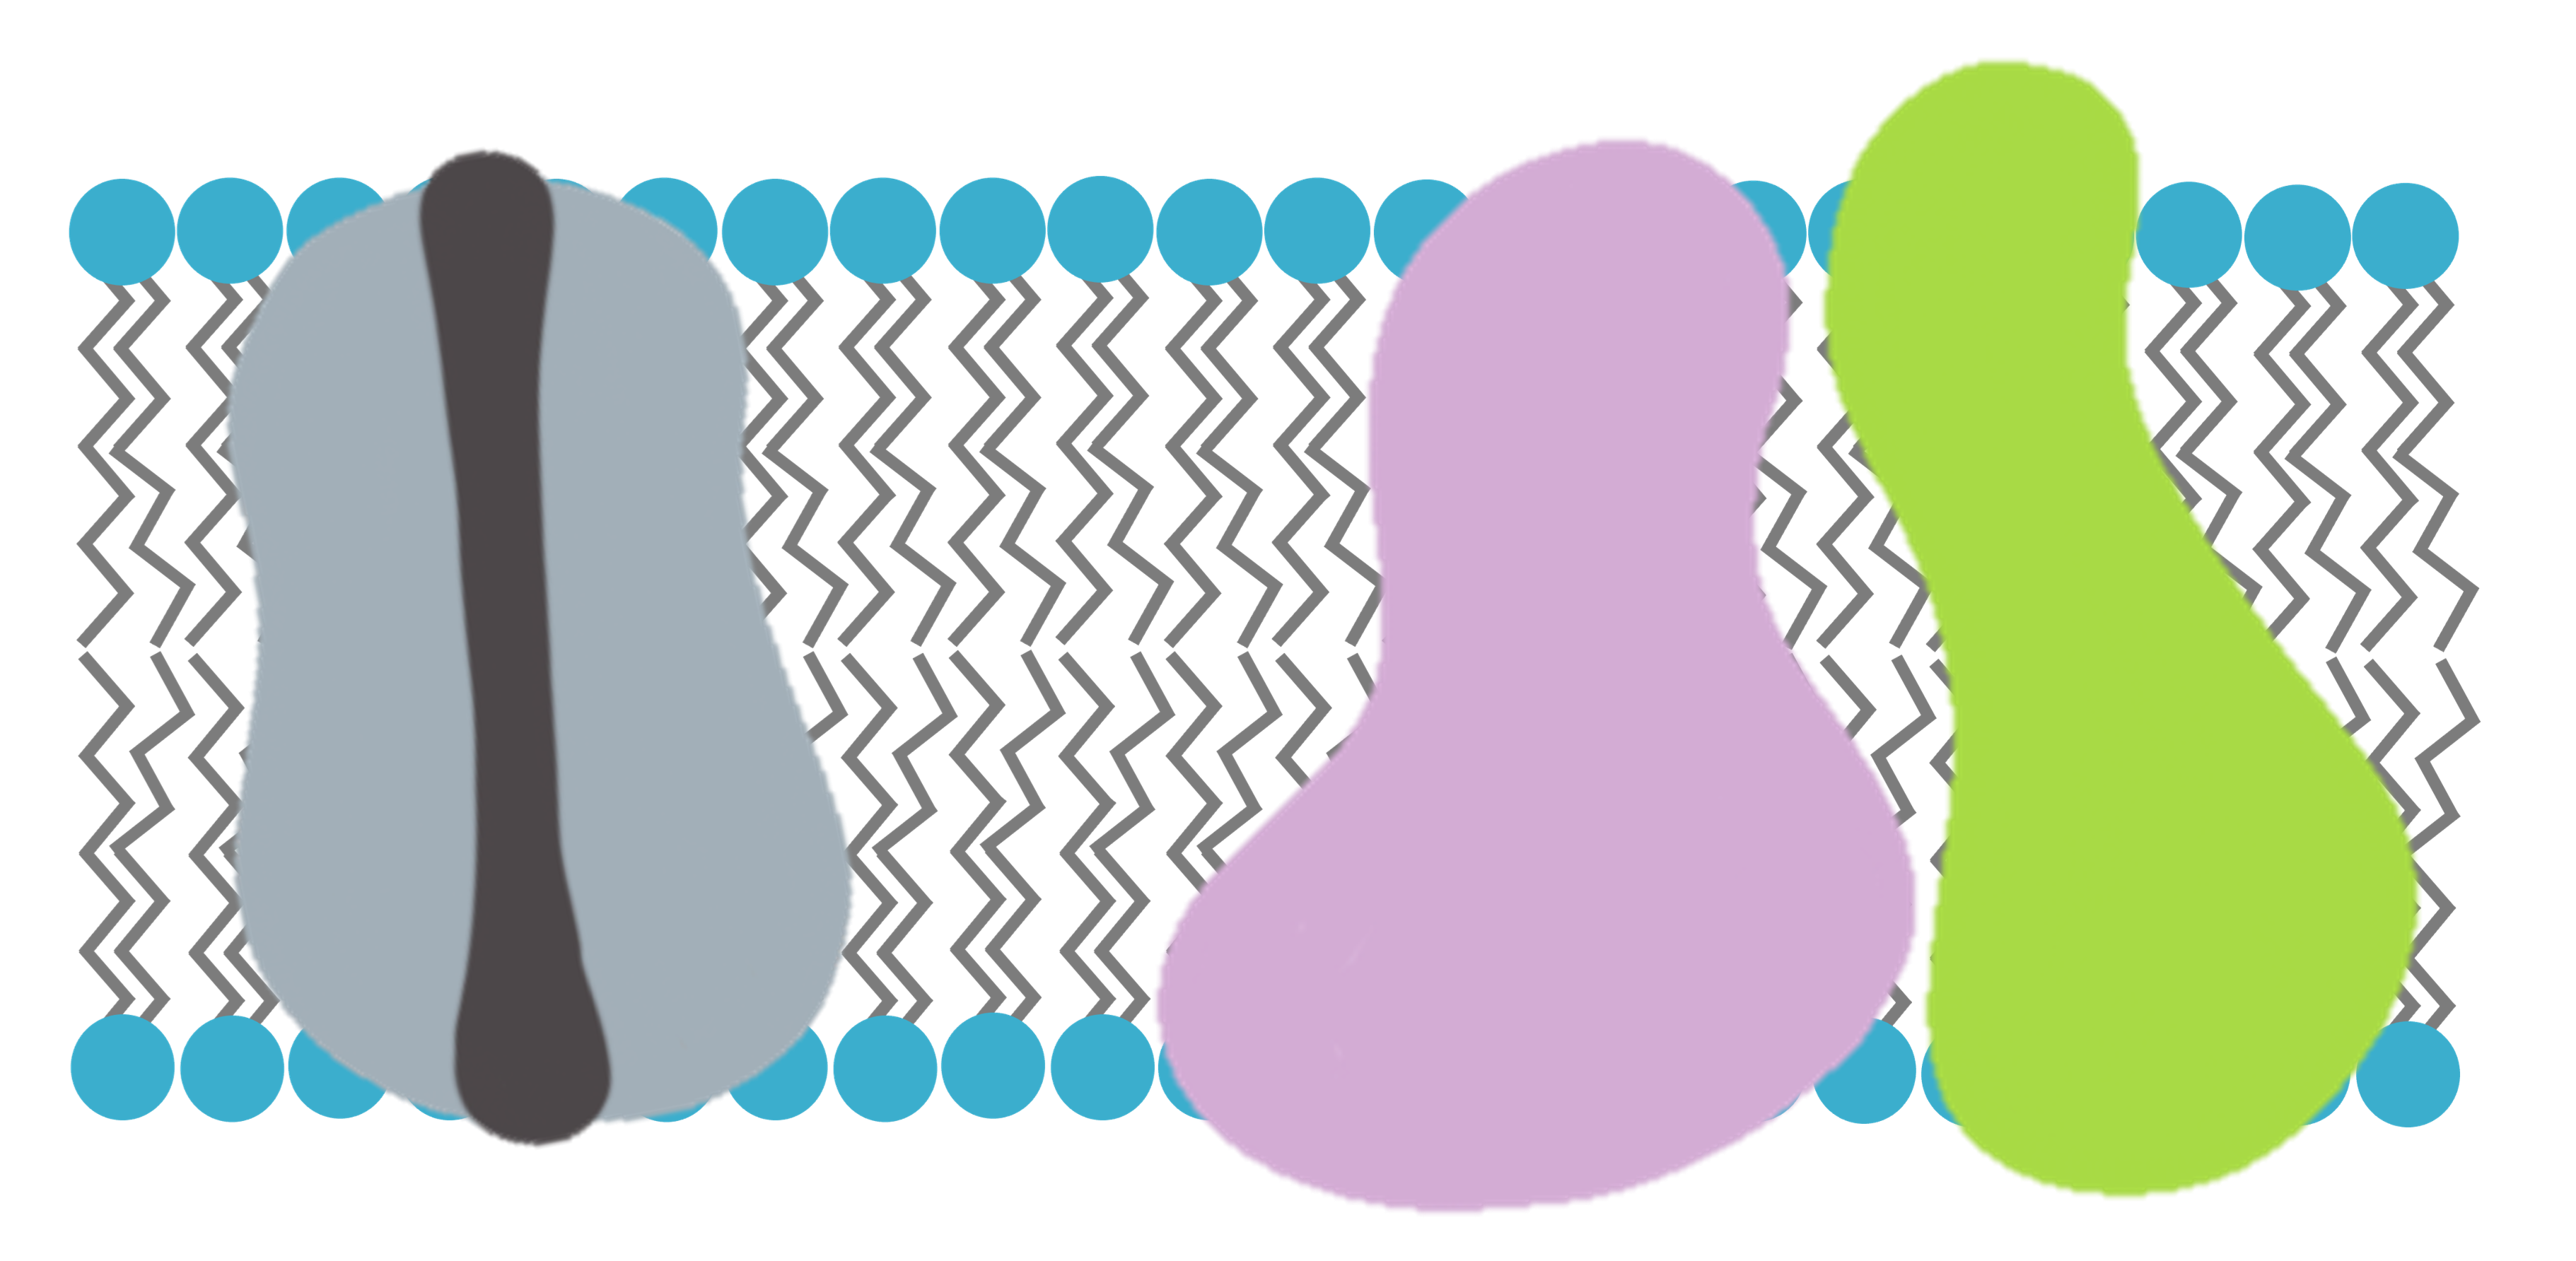
\includegraphics[scale=0.55]{images/proteins embeddings.png} 
    \centering 
    \caption{Rough diagram of proteins embedded in section of cell membrane}
    \centering
\end{figure} 

\subsection*{LC3B} 
\addcontentsline{toc}{subsection}{LC3B} 

For phagophores specifically, I was asked to focus on incorporating LC3B proteins in the membranes of the autophagosome for which I was shared the pdb files of lipidated LC3B. This structure of LC3B has 120 residues with 19 of them being unique. These include: SER, PRO, LYS, ARG, MET, ASP, GLY, TYR, LEU, ALA, PHE, ILE, VAL, THR, ASN, GLU, GLN, HIS and GLP. The GLP residue has resid 120 and one of the important aspects I had to consider while embedding proteins was that this residue must be within the membrane. 

\begin{figure}[h]
    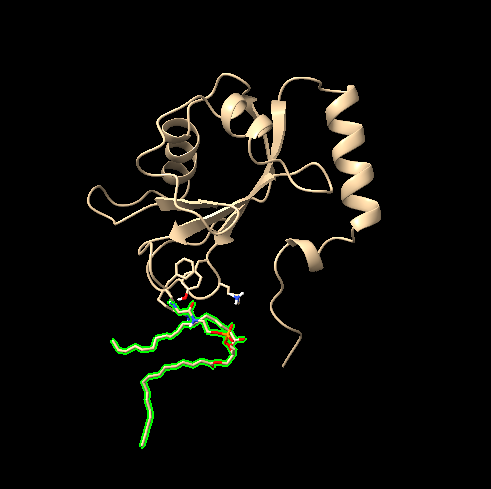
\includegraphics[scale=0.75]{images/lc3b new.png} 
    \centering 
    \caption{Lipidated LC3B at G-120 structure (unbound) with GLP selected}
    \centering
\end{figure} 

\begin{figure}[h]
    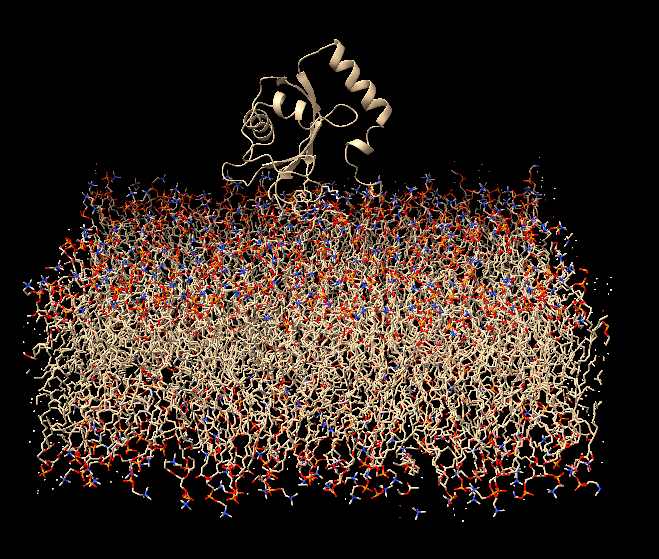
\includegraphics[scale=0.5]{images/lc3b membrane bound.png} 
    \centering 
    \caption{Lipidated LC3B at G-120 structure (membrane bound)}
    \centering
\end{figure} 

\clearpage
\newpage
\section*{phagophore-builder} 
\addcontentsline{toc}{section}{phagophore-builder} 

This Python script was originally written by Dr. Daniel Holdbrook and worked on by Dr. Thukral and her team. I was asked to add functionality to this script to enable the users of this tool to have LC3B proteins as part of their phagophores as well. This tool is meant to be a web-based tool that biologists around the world, with little to no understanding of programming or terminal line commands can use easily to build and view phagophores at different stages of formation, with their desired number of proteins embedded in the membrane. I was thus required to understand what the different functions in the script do and how the final output pdb is created, so that I may write the function to add proteins to the membranes, taking only the number of proteins as inputs from the user. 
\\~\\
\begin{figure}[h]
    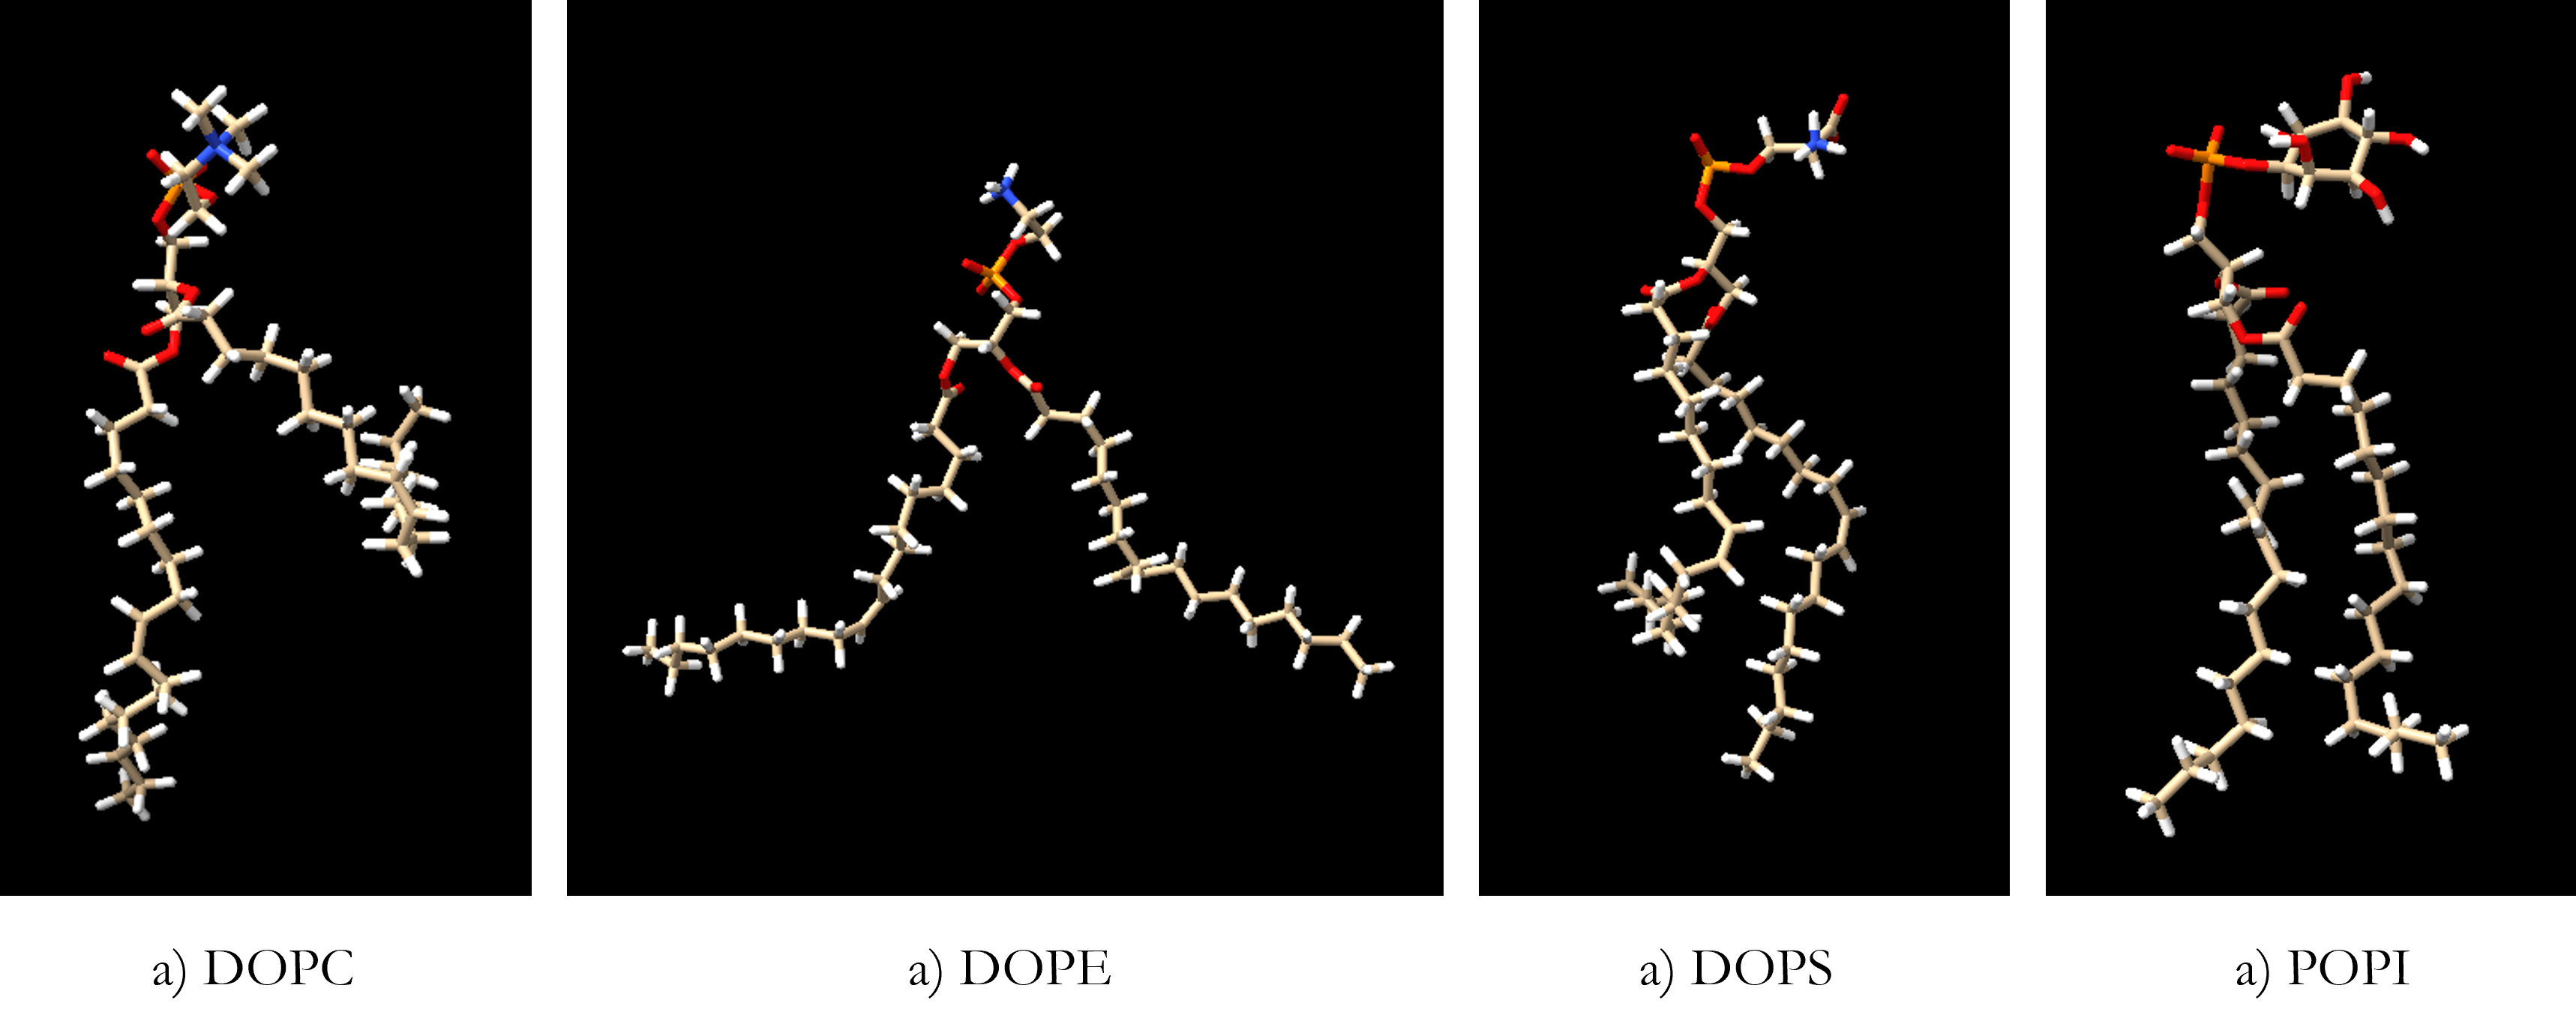
\includegraphics[scale=0.55]{images/phagophore lipids.png} 
    \centering 
    \caption{Lipids used in phagophore-builder}
    \centering
\end{figure} 
\\
The script uses 4 lipids to build the membranes whose ratios are specified as a separate parameter (similar to the composition of the ER membrane from which autophagosomes are thought to originate), according to which they are placed along the phagophore: 
\begin{enumerate}
    \item DOPC : 65\% 
    \item DOPE : 20\% 
    \item DOPS : 5\% 
    \item POPI : 10\%
\end{enumerate}
The script can run on both atomistic as well as CG lipids, and takes their pdb/gro files as inputs. The other parameters it requires are: inner vesicle radius, distance between vesicles, distance between leaflets, area per lipid, slice angle and cone angle. The points on the membrane that need to be populated by lipids are then generated by build functions and saved in a dictionary (results). This information is later merged (using MDAnalysis.Merge) and written to an output pdb file. 
\\~\\

\begin{figure}[h]
    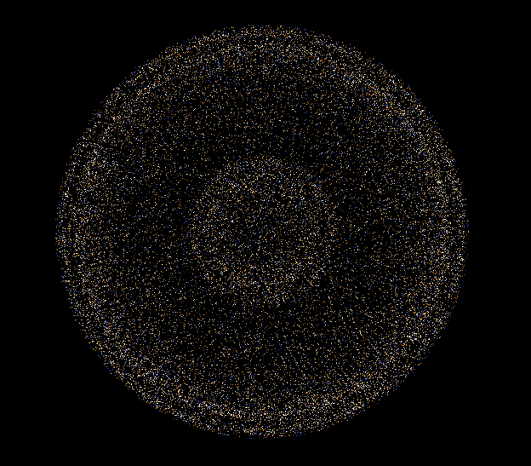
\includegraphics[scale=1]{images/cg full.png} 
    \centering 
    \caption{Complete phagophore built with CG lipids}
    \centering
\end{figure} 

The primary functions used are: 
\begin{enumerate}
    \item reduce\_structure3D(): Takes the lipid input files and generates temporary files for each, with the average radius of the molecules reduced
    \item getLipidList(): Uses the pre-defined ratios of the 4 lipids to generate a list of the required total number of lipids that satisfies the composition constraints (called each time a component of the phagophore is built) 
    \item pointsOnSphere(): Returns a 2D array of coordinates of the desired number of evenly spread out points on a unit sphere (these coordinates are later modified by simply multiplying the desired radius) 
    \item pointsOnTorus(): This generates 2 2D arrays of coordinates on a torus with given slice angle 
    \item build\_cap(): Builds the torus cap for the phagophore by calling pointsOnTorus() twice (builds 2 hollow half tori with different dimensions) and saving the lipid data with their modified coordinates in results["cap"] (called only if both slice and cone angle are not 0) 
    \begin{figure}[h]
    \includegraphics[scale=0.65]{images/torus cap 2 views new.png}
    \centering 
    \caption{Isolated torus cap of phagophore}
    \centering
\end{figure} 
    \item build\_inner\_membrane(): Builds the inner membrane by calling pointsOnSphere() twice (once for each leaflet), modifying lipid coordinates based on the cone angle and saving the results in results["inner"] 
    \item build\_outer\_membrane(): Builds the inner membrane by calling pointsOnSphere() twice (once for each leaflet), modifying lipid coordinates based on the cone angle and saving the results in results["outer"] 
    \item merge\_segments(): Merges atom data in different list entries into one (called at the end of each build function)
    \item merge\_components(): Merges atom data of different components from the results dictionary into one, saving the results in results["final\_model"] (called only once in main() at the end) 
\end{enumerate}

\begin{figure}[h]
    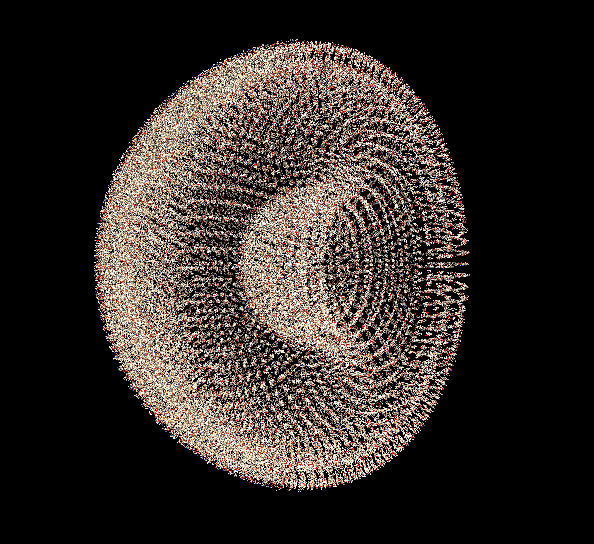
\includegraphics[scale=0.8]{images/half phagophore.png} 
    \centering 
    \caption{Partially formed phagophore with atomistic lipids}
    \centering
\end{figure} 

\clearpage
\newpage 
\section*{Embedding Proteins} 
\addcontentsline{toc}{section}{Embedding Proteins} 

For embedding LC3B in the phagophores generated by the script I worked with the unbound lipidated LC3B pdb file after gaining an understanding of how the script functions with the following stages: 

\subsection*{Stage 1} 
\addcontentsline{toc}{subsection}{Stage 1} 

I started by adding only one protein to the output pdb, to understand how reduce\_structure3D() and MDAnalysis.Writer work. For this, modifications were made to merge\_components() to incorporate proteins into the final model, such that if a proteins keyword exists in the keys of the results dictionary, this information is merged into the final model: 
\\~\\
results["final\_model"] = MDAnalysis.Merge(results["final\_model"].select\_at-
\\oms("all"), results["proteins"].select\_atoms("all")) 
\\~\\ 

reduce\_structure3D() was written in a way as to ignore the chainID while reading a pdb file and hence, all the temporary lipid pdbs that were generated by the function had no chain information and the final pdb had a default chainID of 'M'. This made it impossible to select the proteins separate from the lipids and hence some changes were made to the reduce\_structure3D(), so that chainID would be read from the protein pdb file. This was done by adding an argument called 'flag' to the function. Flag is passed as 0 when the function is being called on a lipid and as 1 when being called on a protein, in which case, the chainID information from the original pdb is also imported to the temp file created.

\begin{figure}[h]
    \centering
    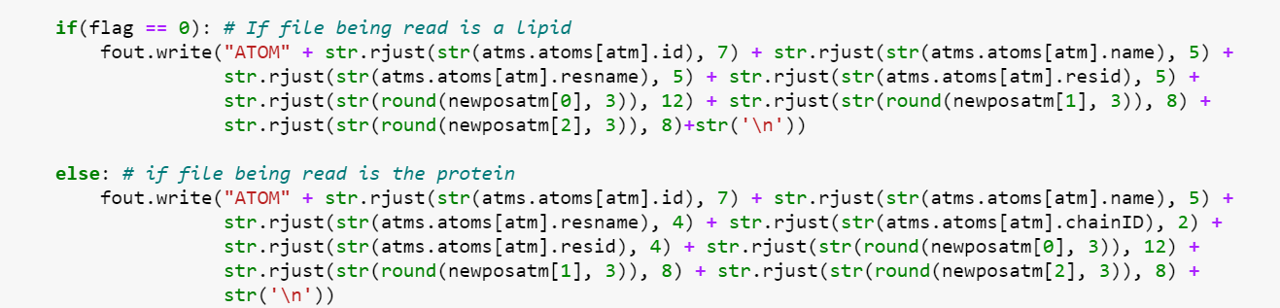
\includegraphics[scale=0.45]{images/reduce.png} 
    \centering 
    \caption{Modifications in reduce\_structure3D} 
\end{figure} 

The LC3B file had residues with resids from 1 - 120, and since these would be added before the lipids, the first resid for the lipid would start from 121. Hence, at this stage, a few lines of code were added to ensure that the residue\_counter value gets updated, by adding to it, the max resid of the protein residues:
\\~\\
u = MDAnalysis.Universe('LC3B.pdb') 
\\ 
results["residue\_counter"] += max(u.atoms.residues.resids)



\subsection*{Stage 2} 
\addcontentsline{toc}{subsection}{Stage 2} 

I then focused on placing proteins on the spherical parts of the membrane, based on a method explained in the paper 'How to generate equidistributed points on the surface of a sphere' by Markus Deserno as shown here: 
\begin{figure}[h]
    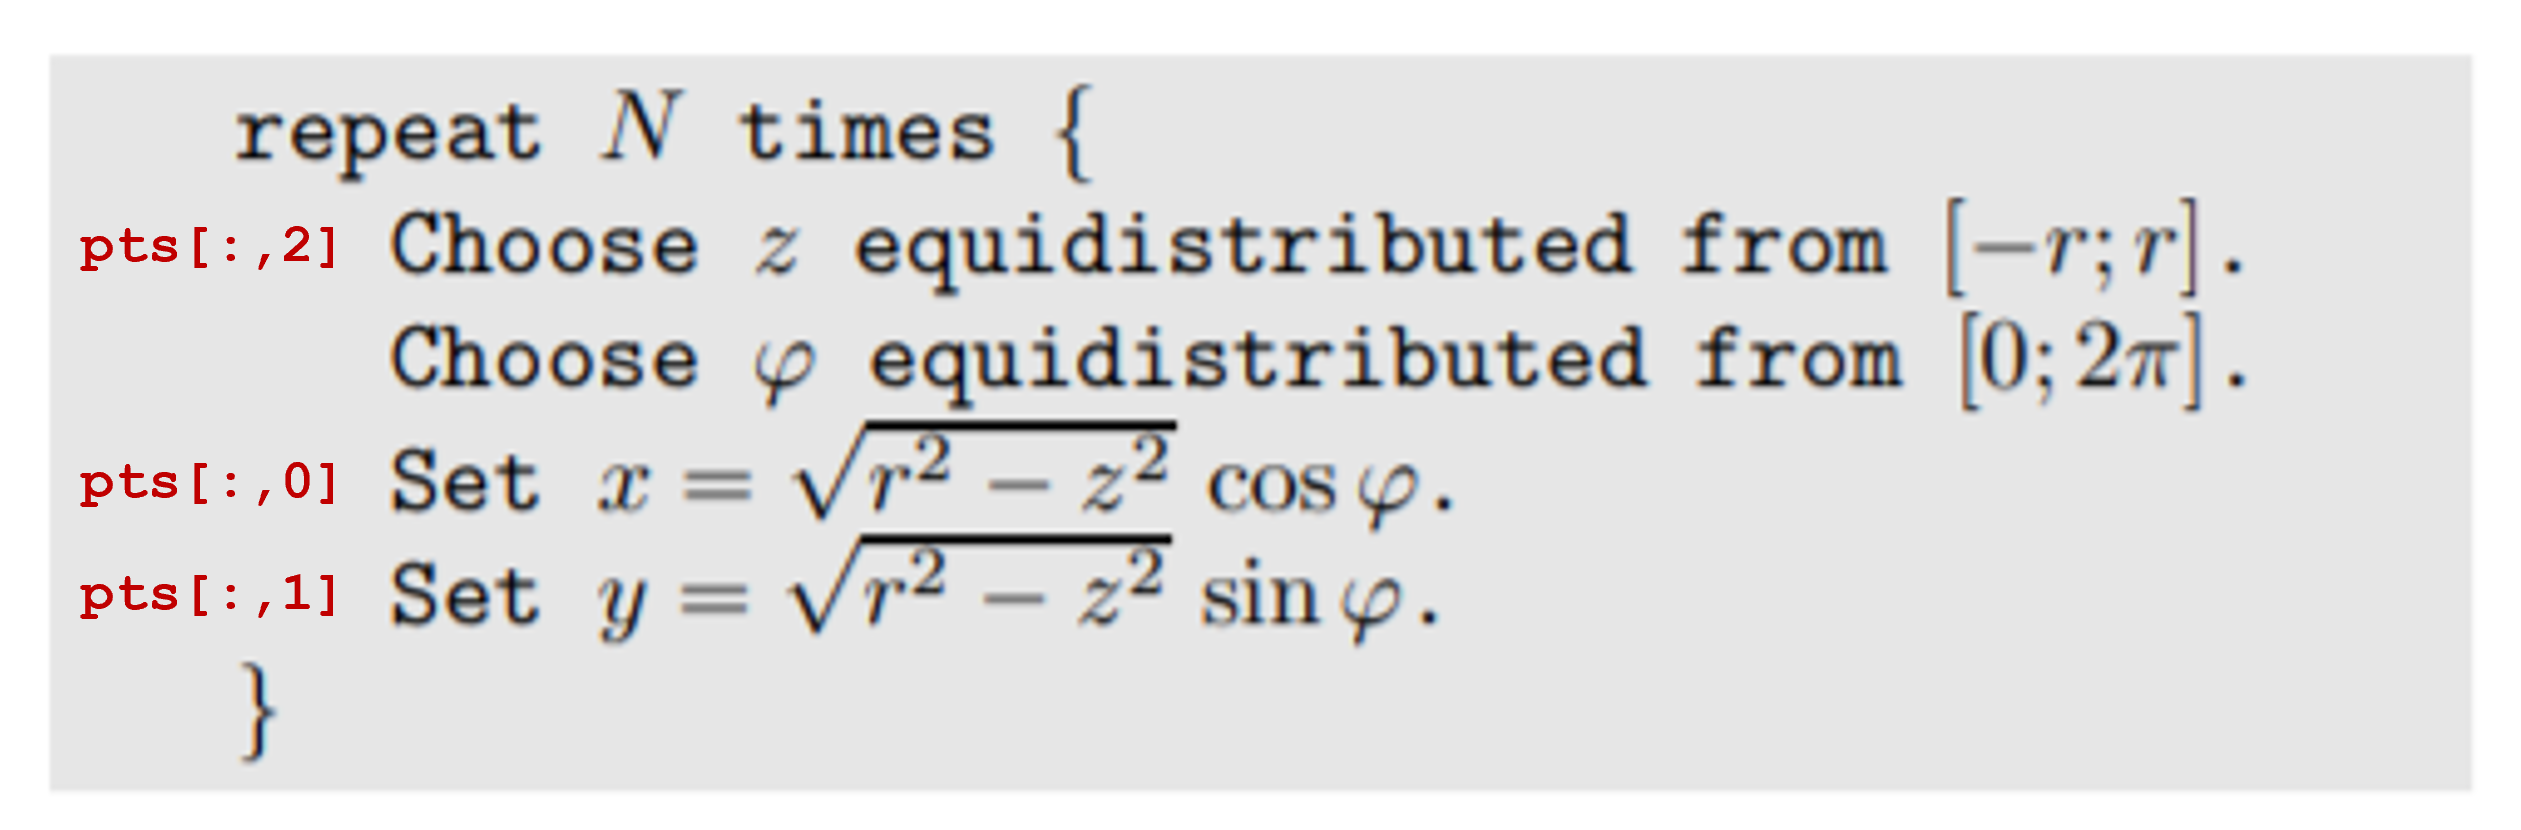
\includegraphics[scale=0.76]{images/deserno.png} 
    \centering 
    \caption{One method of getting equidistributed points on a  sphere adapted from an explanation in above-mentioned paper}
    \centering
\end{figure} 

It was thus implemented as above, returning an nx3 2D array of coordinates for points on a unit sphere (later multiplied by the required radius). numpy.linspace was used to obtain points at regular intervas in a given range: 
\\~\\ 
pts[:, 2] = numpy.linspace(numpy.cos(cone\_ang), -1, num = number\_of\_proteins) 
\\ 
phi = numpy.linspace(0, 2 * numpy.pi, num = number\_of\_proteins) 
\\~\\ 

In the case of a partially formed phagophore, a torus cap is created after a z-coordinate of cos(cone\_ang) is reached and thus, the spherical parts of the phagophore are also not completely formed. Keeping this in mind, constraints were applied to the z coordinates of the returned points, ensuring that these values are between -1 and cos(cone\_ang). 
\\~\\ 

Though this method worked well for small values of number\_of\_proteins, since it was written using numpy.linspace, the arrangement for greater values showed a clear spiral which looked odd and unnatural. 
\\~\\ 
\begin{figure}[h]
    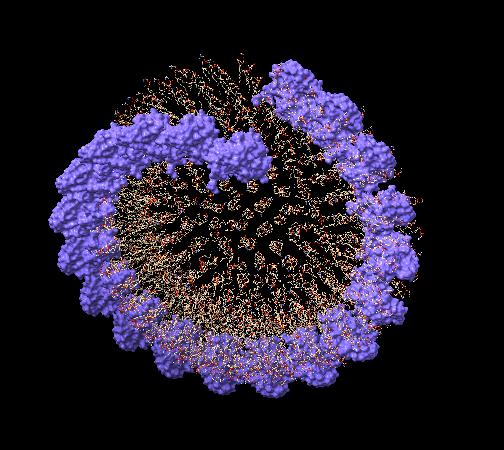
\includegraphics[scale=1]{images/first impl 20.png} 
    \centering 
    \caption{20 proteins placed on a semi-sphere using the above method to generate coordinates}
    \centering
\end{figure} 

\clearpage
\subsection*{Stage 3} 
\addcontentsline{toc}{subsection}{Stage 3} 

Seeing the limitations of my previous method of generating points on a protein, I tried implementing the Fibonacci Lattice method, which functions as follows: 
\begin{enumerate}
    \item Calculates n values of z coordinates, from range cos(cone\_ang) to -1, using numpy.linspace 
    \item Calculates angle $\phi$ by taking the inverse cosine of the z coordinates
    \item Uses z values to calculate intermediate values i 
    \item Calculates angle $\theta$ using array i and the value of the golden ratio 
    \\~\\ 
    Golden ratio = \( \frac{1 + \sqrt{5}}{2}\) = 1.618
    \item Calculates the x and y coordinates finally, using both $\phi$ and $\theta$ where: 
    \\
    x = \sin$\phi$ x \cos$\theta$
    \\
    y = \sin$\phi$ x \sin$\theta$ 
    \\
    z = \cos$\phi$
\end{enumerate}
\\ 
\begin{figure}[h]
    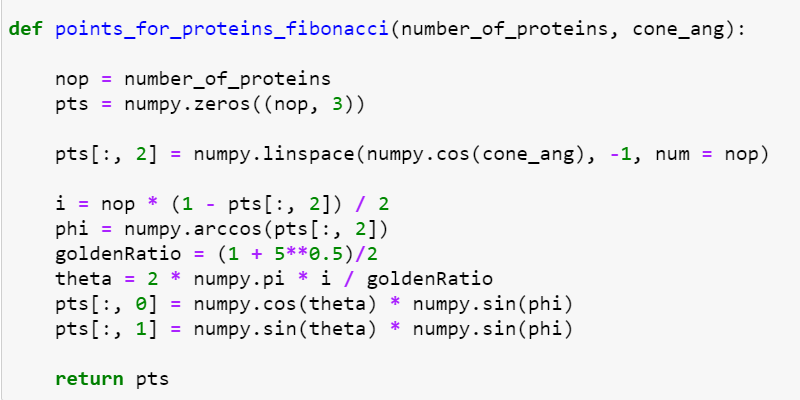
\includegraphics[scale=0.7]{images/fibonacci method.png} 
    \centering 
    \caption{Python implementation of Fibonacci Lattice method for generating equidistant points on the surface of a sphere}
    \centering
\end{figure} 

\\~\\
Though the output with this for intermediate values like 20 looked better than the implementation before, the result still looked strange and unlike what one would expect the distribution of proteins to be like on an actual phagophore. This method is known to work best for generating equidistant points for very large values of n. 
\\~\\ 
\begin{figure}[h]
    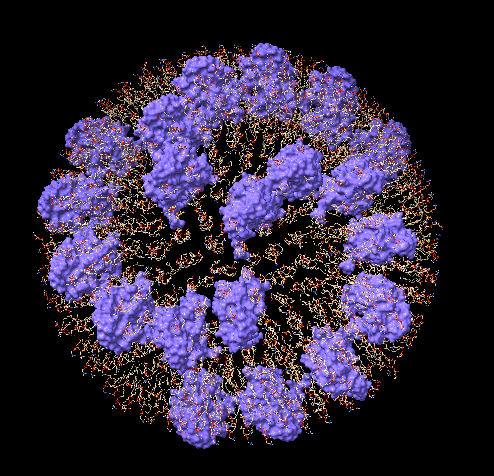
\includegraphics[scale=1]{images/fibonacci 20.png} 
    \centering 
    \caption{20 proteins placed on a semi-sphere using the Fibonacci Lattice method to generate coordinates}
    \centering
\end{figure} 

\clearpage 
Finally, using the pointsOnSphere() function already defined in the script by Dr. Holdbrook (generates equidistant points on the entire surface area of a sphere), I wrote a new function to generate equidistant points on a sphere or a part of it. 
\begin{figure}[h]
    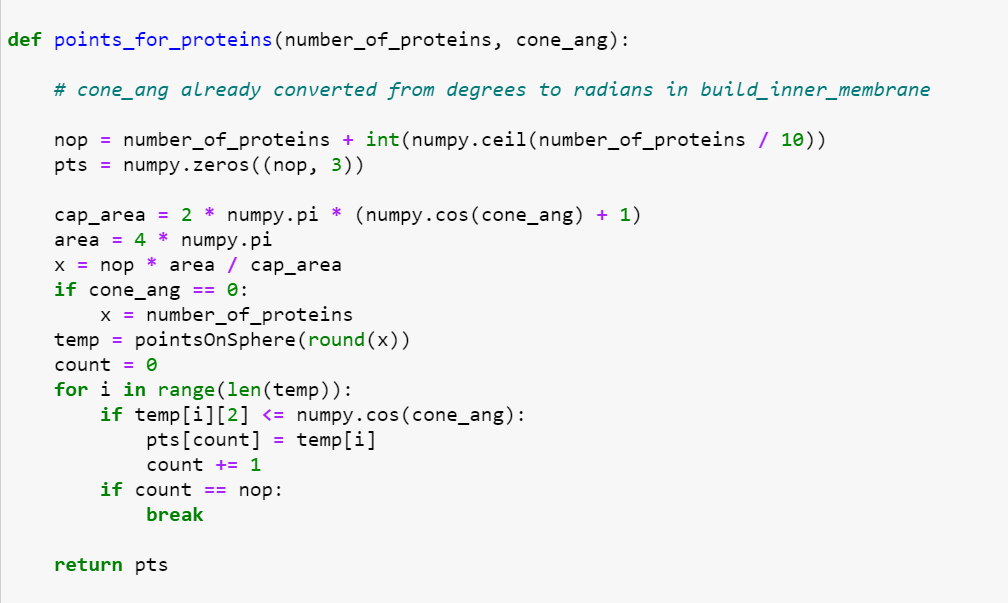
\includegraphics[scale=0.55]{images/final implementation.png} 
    \centering 
    \caption{Final implementation of points\_for\_proteins() function}
    \centering
\end{figure} 

This function works as follows: 
\begin{enumerate}
    \item Takes number\_of\_proteins and cone\_ang as arguments 
    \item Sets variable nop as \( \frac{11}{10}\) x number\_of\_proteins  
    \item Calculates area of the spherical cap or part of the sphere being worked with using cone\_ang and total area of sphere (assuming unit radius) 
    \\~\\
    \(A\) = \( \frac{3}{r}\)\(V_{spherical Cap}\) = \( \frac{3}{r}\)\( \frac{1}{3}\)\({2$\pi$r^2h}\)  = \(2$\pi$rh\) 
    \item Using ratio of areas, calculates value of variable \(x\) as the total number of points on a whole sphere if nop points were spread out evenly on a part of the sphere (if a whole sphere itself is being used, as in the case of building a fully formed phagophore, the value of x is set to nop itself) 
    \item Obtains coordinates for \(x\) points by calling pointsOnSphere() 
    \item Returns a 2D array of coordinates on the sphere where z coordinate is less than numpy.cos(cone\_ang) 
\end{enumerate}

\begin{figure}[h]
    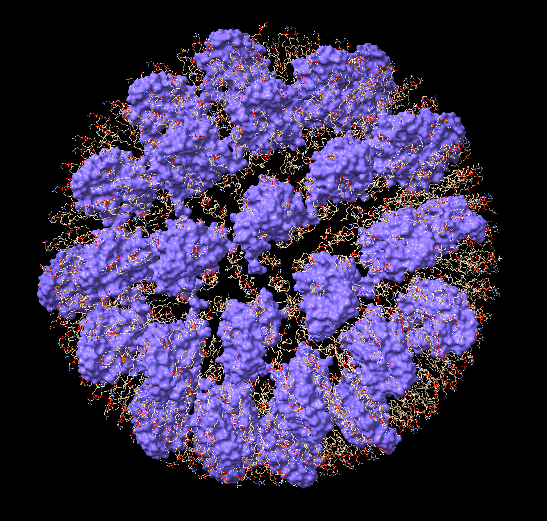
\includegraphics[scale=1]{images/final impl 28.png} 
    \centering 
    \caption{20 proteins placed on a semi-sphere using the above method to generate coordinates}
    \centering
\end{figure} 

\clearpage
\subsection*{Stage 4} 
\addcontentsline{toc}{subsection}{Stage 4} 

I now moved on to fixing the position of the GLP residue (with resid 120) and the embedding of the protein as a whole in the membrane. The protein must be so positioned that only the GLP residue is within the outer boundaries of the 2 leaflets of the membrane, with the rest of the protein being outside it. For this, the length of the GLP length was calculated by: 

\begin{enumerate}
    \item Getting the positions of the atoms of the GLP chain 
    \item Getting the positions of the top and bottom atoms in this list 
    \item Calculating the length of the chain using Euclidean distance: 
    \\~\\
    \(length\) = \sqrt{\((x_2 - x_1)^2 + (y_2 - y_1)^2 + (z_2 - z_1)^2\)}
\end{enumerate} 
and added to the radius while positioning proteins. 

\begin{figure}[h]
    \includegraphics[scale=0.6]{images/glp chain.png} 
    \centering 
    \caption{Positioning of protein and G-120 residue}
    \centering
\end{figure} 

In a double-membrane vesicle, the proteins on the inner membrane are oriented towards the center, with their heads within the vesicle instead of their heads being in the inter-membrane cavity. For this, the atoms for inner membrane proteins were rotated by 180$\degree$ using the following MDAnalysis function: 
\\ 
atomsel.rotateby(180, atomsel.principal\_axes()[0]) 

\begin{figure}[h]
    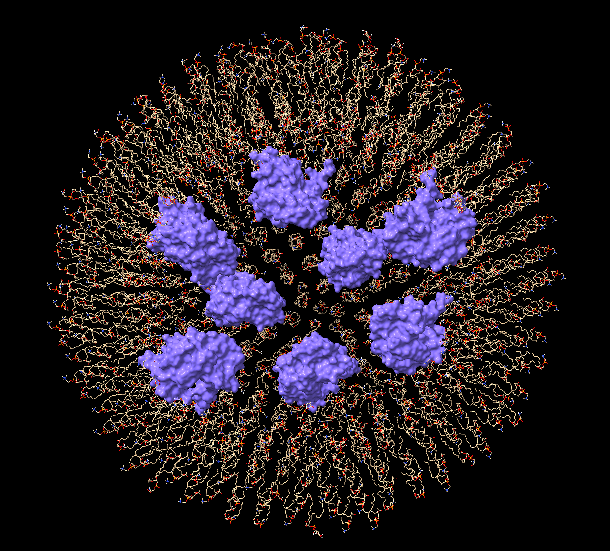
\includegraphics[scale=0.9]{images/inner membrane p.png} 
    \centering 
    \caption{Inner membrane proteins oriented towards the center}
    \centering
\end{figure} 

\clearpage
\subsection*{Stage 5} 
\addcontentsline{toc}{subsection}{Stage 5} 

While adding proteins, the proteins may get placed at the same positions as some of the lipids, causing steric clashes. The proteins may also clash with other proteins already added to the system. I thus added code to check for clashes each time a lipid is being added (after it is properly rotated and translated), in functions build\_inner\_membrane() and in build\_outer\_membrane(), committing the changes only if there are no clashes. 
\\~\\
\begin{figure}[h]
    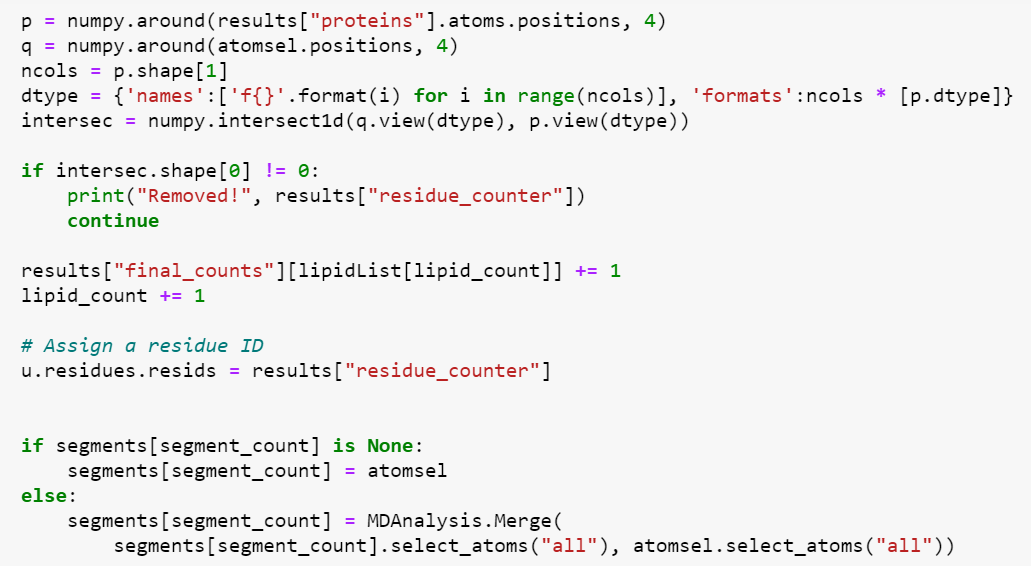
\includegraphics[scale=0.57]{images/checking for clashes.png} 
    \centering 
    \caption{Code implemented for checking for clashes between lipids and proteins}
    \centering
\end{figure} 

\\~\\
The code works as follows: 
\begin{enumerate}
    \item Takes positions of proteins already added as set p and positions of current lipid as set q (these values are kept as is for now and this does not cause any clashes, but may be rounded off to an appropriate number of decimal places if necessary) 
    \item Calculates the intersection of the two sets using numpy.intersect1d and creating a new data type for an array of dimensions 1x3 with float32 values 
    \item If first dimension of intersection set is not 0 i.e. $\ge$ 1 atom from the lipid being added has the same coordinates as some protein that has already been added, the lipid is skipped (proceeds to next iteration of for loop) 
    \item If not, resids of lipid and results[“final\_counts”] are modified and the lipid information is added to segments 
\end{enumerate} 

Since this checks for clashes with lipids as the lipids are being added to the system, proteins need to be added before any build functions are called. 
\\~\\ 
A similar process is followed within the add\_proteins function, where clashes are checked for using the positions of the current protein being added, and all the proteins that have already been added to the system. 
\\~\\
\begin{figure}[h]
    \includegraphics[scale=0.5]{images/full images of partial phagophore.png} 
    \centering 
    \caption{Partially formed phagophore with cone\_ang = 92.5 \degree and 10 proteins on the outer membrane}
    \centering
\end{figure} 

\subsection*{Stage 6} 
\addcontentsline{toc}{subsection}{Stage 6} 

I finally focused on adding points to the torus cap. build\_cap() calls pointsOnTorus() twice: 
\begin{enumerate}
    \item To build the outer torus cap, with outer radius as cap\_rad2 and inner radius as cap\_rad1, defined as follows: 
    \\~\\ 
    cap\_rad1 = parameters["inner\_vesicle\_radius"] - 
        \\ (parameters["dist\_bw\_leaflets"] / 2)
    \\~\\
    cap\_rad2 = parameters["inner\_vesicle\_radius"] + 
        \\ (parameters["dist\_bw\_leaflets"] / 2) + parameters["dist\_bw\_vesicles"] 
    \item To build the inner torus cap, with outer radius as torus\_rad2 and inner radius as torus\_rad1, defined as follows: 
    \\~\\ 
    torus\_rad1 = parameters["inner\_vesicle\_radius"] + 
        \\ (parameters["dist\_bw\_leaflets"] / 2)
    \\~\\
    torus\_rad2 = parameters["inner\_vesicle\_radius"] - 
        \\ 
        (parameters["dist\_bw\_leaflets"] / 2) + parameters["dist\_bw\_vesicles"] 
\end{enumerate}


I started off with choosing points on the outer torus cap by simply using numpy.linspace. This, however, caused the protein placement to look odd. Thus I focused on generating circles of increasing radii, starting with the inner radius of the outer torus cap, and with increasing z, staring with cos(cone\_ang), with an appropriate step value: 
\\~\\ 
\begin{figure}[h]
    \centering 
    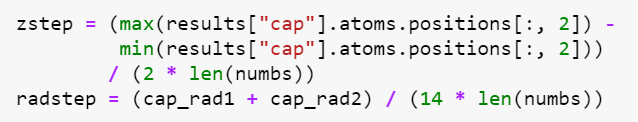
\includegraphics[scale=0.9]{images/steps in torus.png} 
    \centering 
    \caption{Step values for the z-coordinate and the radius of the circle for generating points on a torus} 
\end{figure} 
\\~\\
The code thus works as follows: 
\begin{enumerate}
    \item Divides the number of proteins that need to be placed on the torus into smaller sets 
    \item Using numpy.linspace, generates x and y coordinates on a circle with the current selected radius 
    \\~\\ 
    theta = numpy.linspace(0, 2 * numpy.pi, num = n) 
    \\
    pts[:, 0] = numpy.cos(theta) 
    \\
    pts[:, 1] = numpy.sin(theta) 
    \item Uses the above defined step values to calculate current radius and z coordinate (using 'p', the loop iteration number) and thus modifies pts 
    \\~\\  
    rad = cap\_rad1 + p*radstep 
    \\ 
    pts *= rad - glp\_length
    \\ 
    pts[:, 2] = numpy.cos(cone\_ang) + p * zstep
\end{enumerate} 

\begin{figure}[h]
    \includegraphics[scale=0.45]{images/torus proteins.png} 
    \centering 
    \caption{9 points placed in 3 rings of 3 in the inner section of a torus}
    \centering
\end{figure} 

\clearpage
\newpage 
\section*{Summary} 
\addcontentsline{toc}{section}{Summary} 

I thus developed changes for reduce\_structure3D() and merge\_components() along with build\_inner\_membrane() and build\_outer\_membrane(). While committing my changes however, I excluded the modifications and call to reduce\_structure3D(), as the output was the same without it. The main functionality of adding proteins takes place in the add\_proteins() function, whose process is explained here: 

\begin{enumerate}
    \item Takes parameters dictionary, protein file name, number of inner membrane proteins (number\_inner), number of outer membrane proteins (number\_outer) and results dictionary as parameters 
    \item Calculates length of GLP-120 chain using Euclidean distance and saves the value in glp\_length 
    \item Calculates coordinates for proteins saved in an nx3 dimension array by calling points\_for\_proteins 
    \item Creates an MDAnalysis universe of the given protein and rotates and translates according to coordinates generated previously 
    \item Checks for clashes by using the same procedure as before (compares coordinates of current protein and proteins already added to current segments entry) 
    \item In case of no clashes, the protein is added to the current segments entry by calling add\_to\_segment() and the count of proteins added is incremented 
    \item Steps 3 to 6 are repeated for number\_inner and number\_outer 
    \item For inner membrane proteins, radius of sphere is taken to be 
    \\parameters["inner\_vesicle\_radius"] - (parameters["dist\_bw\_leaflets"] / 2) - glp\_length 
    \\and proteins are rotated by 180 degrees before translation 
    \item For outer membrane proteins, radius of sphere is taken to be 
    \\parameters["inner\_vesicle\_radius"] + (parameters["dist\_bw\_leaflets"] / 2) + parameters["dist\_bw\_vesicles"] + glp\_length 
    \item Finally, results[“residue\_counter”] is updated and merged segments are added to results[“proteins”] 
\end{enumerate}

\clearpage
\newpage 
\section*{Results} 
\addcontentsline{toc}{section}{Results} 

The code I have written thus adds LC3B proteins to the membranes of the phagophores created by the script phagophore-builder. The proteins are made select-able as chain 'A' in Chimera as well, separate from the lipids added, and are oriented with just the GLP residue embedded in the membrane. 
\\~\\
LC3B proteins are added to the spherical components of the phagophore i.e. the spherical inner and outer membranes, and are equally distributed over the whole surface, and not clustered randomly. These proteins are added according to the inputs of the user, where the user specifies the number of proteins required for each section. The proteins on the inner membrane are oriented inwards, towards the vesicle cavity. 
\\~\\
For the torus, proteins are added to the inner section, in an equi-distributed manner, placed on circles of increasing radius, with their heads oriented inwards. Further changes still need to be made to this function, to ensure that the proteins are placed with sufficient distance between them. 

\newpage
\section*{Bibliography} 
\addcontentsline{toc}{section}{Bibliography} 


\begin{enumerate}
    \item CSIR Official Website: 
    \\https://www.csir.res.in/about-us/about-csir 
    \item IGIB Official Website: https://www.igib.res.in/  
    \item MARTINI Force Field Parameters, Lipids: http://cgmartini.nl/index.php/
    \\force-field-parameters/lipids 
    \item Britannica, Lipid Bilayer: https://www.britannica.com/science/lipid-bilayer 
    \item Jing, Kaipeng, and Kyu Lim. “Why is autophagy important in human diseases?.” Experimental & molecular medicine vol. 44,2 (2012): 69-72. doi:10.3858/emm.2012.44.2.028 
    \item Britannica, Autophagocytosis: https://www.britannica.com/science/
    \\autophagocytosis 
    \item Bernard, Amélie, and Daniel J Klionsky. “Autophagosome formation: tracing the source.” Developmental cell vol. 25,2 (2013): 116-7. doi:10.1016/j.devcel.2013.04.004 
    \item Biazik, Joanna et al. “Ultrastructural relationship of the phagophore with surrounding organelles.” Autophagy vol. 11,3 (2015): 439-51. doi:10.1080/15548627.2015.1017178 
    \item Mari, Muriel et al. “The puzzling origin of the autophagosomal membrane.” F1000 biology reports vol. 3 (2011): 25. doi:10.3410/B3-25
    \item Mizushima, Noboru. “Autophagy: process and function.” Genes & development vol. 21,22 (2007): 2861-73. doi:10.1101/gad.1599207 
    \item Jatana, Nidhi et al. “Human LC3 and GABARAP subfamily members achieve functional specificity via specific structural modulations.” Autophagy vol. 16,2 (2020): 239-255. doi:10.1080/15548627.2019.1606636 
    \item UCSF Chimera, Tutorial:  https://www.cgl.ucsf.edu/Outreach/Tutorials/
    \\GettingStarted.html 
    \item GROMACS, File Formats: https://manual.gromacs.org/documentation/
    \\current/reference-manual/topologies/topology-file-formats.html\#molitp 
    \item Abraham, M. et al. “GROMACS: High performance molecular simulations through multi-level parallelism from laptops to supercomputers.” SoftwareX 1 (2015): 19-25.
    \item GROMACS, Documentation: https://manual.gromacs.org/documentation/
    \\current/onlinehelp/ 
    \item MARTINI, Documentation: http://cgmartini.nl/index.php/about 
    \item MARTINI, Lipid Membranes: http://cgmartini.nl/index.php/example-applications2/lipid-membranes 
    \item Boyd, Kevin J, and Eric R May. “BUMPy: A Model-Independent Tool for Constructing Lipid Bilayers of Varying Curvature and Composition.” Journal of chemical theory and computation vol. 14,12 (2018): 6642-6652. doi:10.1021/acs.jctc.8b00765 
    \item BUMPy, Code Repository: https://github.com/MayLab-UConn/BUMPy 
    \item CHARMM-GUI, Library of Pure Lipid Bilayer: 
    https://www.charmm-gui.org/?doc=archive&lib=lipid\_pure
    \item MDAnalysis, Tutorial: https://www.mdanalysis.org/MDAnalysisTutorial/ 
    \item MDAnalysis, Documentation: https://docs.mdanalysis.org/stable/index.html 
    \item NumPy Documentation, NumPy v1.21 Manual: 
    https://numpy.org/doc/1.21/ 
    \item Deserno, Markus. "How to generate equidistributed points on the surface of a sphere." If Polymerforshung (Ed.) 99.2 (2004). 
    \item Article, 'How to evenly distribute points on a sphere more effectively than the canonical Fibonacci Lattice', 2020. 
    http://extremelearning.com.au/
    \\how-to-evenly-distribute-points-on-a-sphere-more-effectively-than-the-
    \\canonical-fibonacci-lattice/ 
    \item Article, 'Spherical Cap'. https://en.wikipedia.org/wiki/Spherical\_cap 
    
\end{enumerate} 

\end{document}
